\chapter{Fourier-Theorie f"ur die Kugeloberfl"ache
\label{chapter:kugel}}
\lhead{Fourier f"ur die Kugeloberfl"ache}
\begin{refsection}
\chapterauthor{Thomas Gujer und Christoph Schmitz-Dr"ager}

\section{Einleitung}
\rhead{Einleitung}

In diesem Kapitel m"ochten wir veranschaulichen, dass die Effekte 
welche man bei der klassischen Fourier-Theorie beobachten kann, 
auch bei der Fourier-Theorie auf der Kugeloberfl"ache zu sehen sind.
Zur Visualisierung vergleichen wir jeweils ein Rechtecksignal mit 
dem Analogon auf der Kugeloberfl"ache.

\section{Funktionen auf der Kugeloberfl"ache}
\rhead{Funktionen auf der Kugeloberfl"ache}
Im Gegensatz zu den Funktionen welche mittels klassischer 
Fourier-Theorie analysiert werden, besitzen Funktionen auf der 
Kugeloberfl"ache 3 Variablen und einen Funktionswert. 
Da der Funktionswert aber nicht in einer weiteren Dimension 
dargestellt werden kann, muss man auf andere Mittel zur"uckgreifen. 
Das heisst, die 3 Variablen bestimmen die geometrischen Abmessungen 
und der Funktionswert wird mittels Farbschl"ussel dargestellt. 
Dies ist dieselbe Darstellung, welche z.B. auch f"ur die Temperatur 
auf der Erdoberfl"ache verwendet wird. In diesem Fall darf man die 
Form der Erde auch nicht beeinflussen um die Temperatur darzustellen.
\subsection{Kugelkoordinaten}
\begin{figure}%Bild Koordinaten der Kugel
\centering
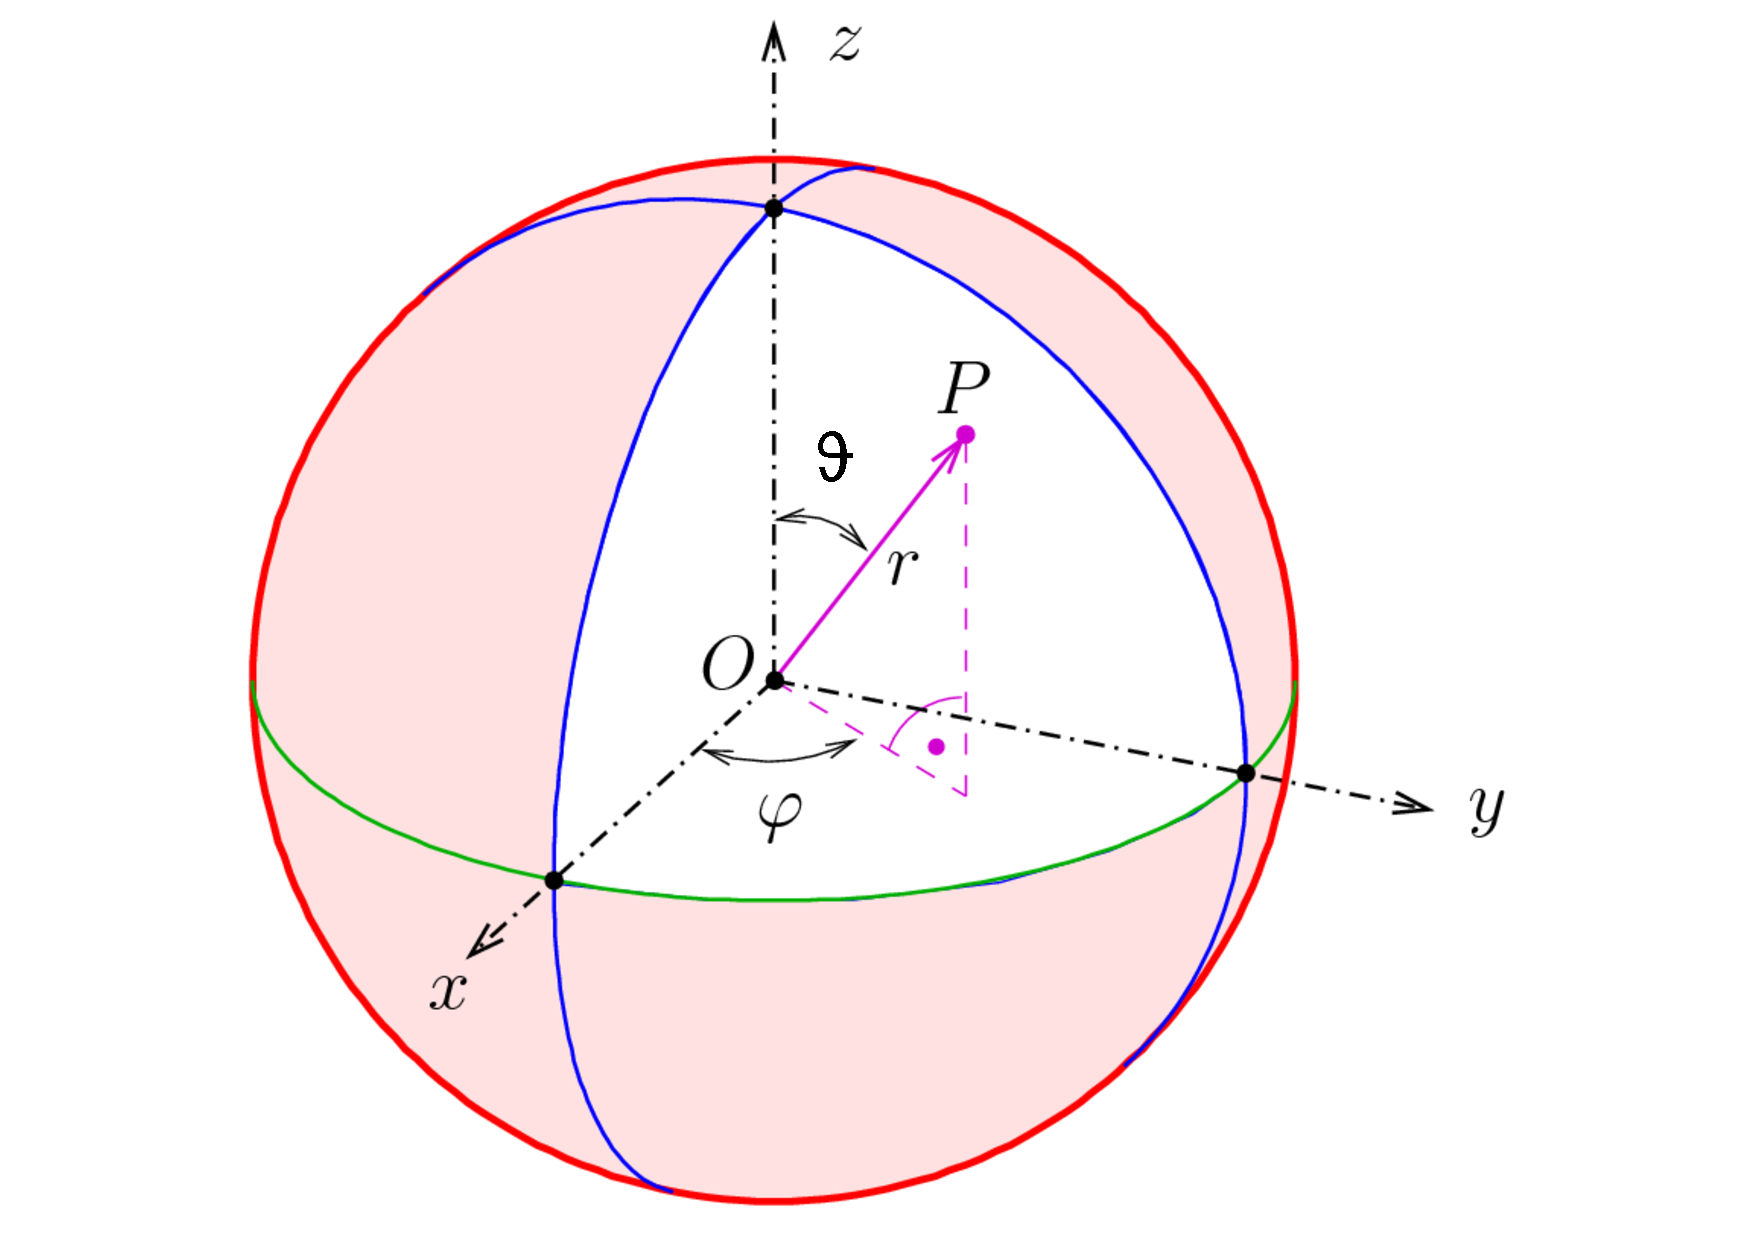
\includegraphics[width=0.7\textwidth]{kugel/Kugelkoord.pdf}
\caption{Koordinaten der Kugel
\label{skript:Koordinaten der Kugel}}
\end{figure}

In der Abbildung \ref{skript:Koordinaten der Kugel} 
ist zu sehen wie ein Punkt auf der Kugeloberfl"ache in 
Polar-Koordinaten definiert ist. 
Zum umrechnen ins kartesische Koordinatensystem werden folgende 
Formeln ben"otigt:
\begin{align*}
x& = r \cdot \sin\vartheta \cdot \cos\varphi 
\\
y& = r \cdot \sin\vartheta \cdot \sin\vartheta
\\
z& = r \cdot \cos\vartheta 
\end{align*}

\subsection{Rechteckfunktionen}
\begin{figure}%Funktion auf Rechteckoberfläche 
\centering
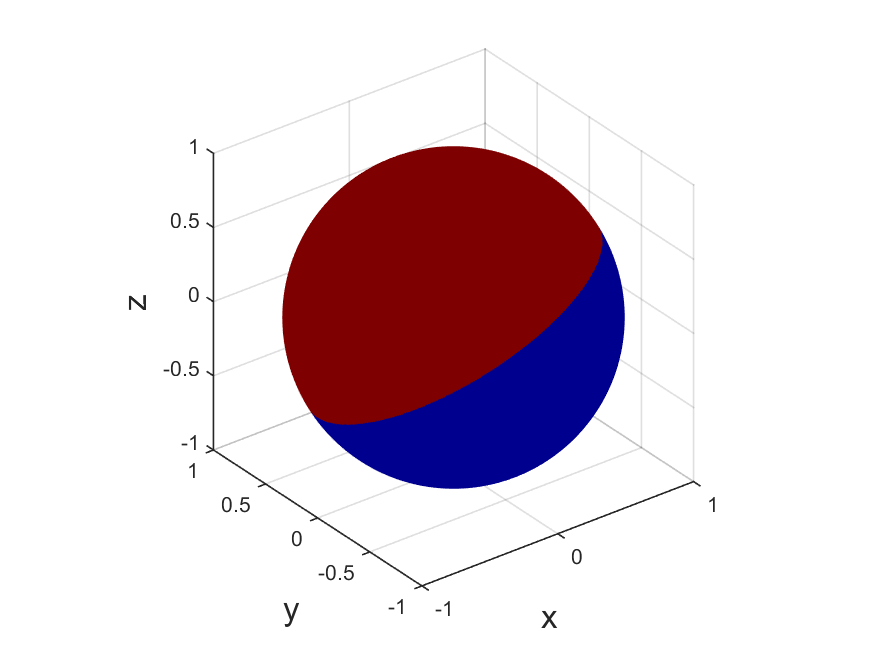
\includegraphics[width=0.7\textwidth]{kugel/Funktion.pdf}
\caption{Funktion auf Kugeloberfl"ache
\label{skript:Funktion auf Kugeloberfl"ache}}
\end{figure}
Die Rechteckfunktion in unseren Beispielen wurde mit den 
Funktionswerten 0 und 1 definiert. 
Die Funktion auf der Kugeloberfl"ache wurde analog 
mit denselben Funktionswerten definiert. 
Dabei wurde einem kreisf"ormigen Abschnitt auf der Kugeloberfl"ache 
der Wert 1 zugewiesen und der Rest der Kugeloberfl"ache besitzt den 
Funktionswert 0. 

Eine Rechteckfunktion ist folgendermassen definiert:
\[
f(x) =
\begin{cases}
1 & \text{wenn } 0 \leq x \leq \pi\\
0 & \text{sonst }
\end{cases}
\]
Das Analogon auf der Kugeloberfl"ache ist folgendermassen definiert:
\begin{enumerate}

\item Definition eines Vektors mit dem Startpunkt im Zentrum der Kugel
und dem Endpunkt auf der Kugeloberfl"ache:

$$
\vec{c} = 
\begin{pmatrix}
{r \cdot \sin\vartheta \cdot \cos\varphi}\\
{r \cdot \sin\vartheta \cdot \sin\vartheta}\\
{r \cdot \cos\vartheta}
\end{pmatrix}
\text{mit r = 1 folgt $\vec{r}$ =}
\begin{pmatrix}
{\sin\vartheta \cdot \cos\varphi}\\
{\sin\vartheta \cdot \sin\vartheta}\\
{\cos\vartheta}
\end{pmatrix}
$$

\item	Des Weiteren wird ein Vektor definiert, welcher den Startpunkt
im Zentrum der Kugel und den Endpunkt auf der Kugeloberfl"ache hat. 
Im Gegensatz zum $\vec{c}$ wo die Winkel $\vartheta$ und $\varphi$ 
eindeutig definiert sind, besitzt der $\vec{r}$ eine variables 
$\vartheta$ von 0 bis $\pi$ und ein variables $\varphi$ von $-\pi$ 
bis $\pi$: 

$$
\vec{r} = 
\begin{pmatrix}
{r \cdot \sin\vartheta \cdot \cos\varphi}\\
{r \cdot \sin\vartheta \cdot \sin\vartheta}\\
{r \cdot \cos\vartheta}
\end{pmatrix}
\text{mit r = 1 folgt $\vec{r}$ =}
\begin{pmatrix}
{\sin\vartheta \cdot \cos\varphi}\\
{\sin\vartheta \cdot \sin\vartheta}\\
{\cos\vartheta}
\end{pmatrix}
$$

\item
\[
f(x,y,z) =\begin{cases}
1 & \text{wenn } \vec c\cdot\vec r \ge 0\\
0 & \text{sonst}
\end{cases}
\]
\end{enumerate}

\section{Fourier-Theorie}
\rhead{Fourier-Theorie}

\subsection{Kugelfl"achenfunktionen}
Kugelfl"achenfunktionen sind die Analoga zu den Sinus- und 
Kosinus-Funktionen bei der klassischen Fourier-Theorie. 
Mittels dieser Kugelfl"achenfunktionen $Y_{lm}$ und $Z_{lm}$ 
bildet man ein orthogonales System von Funktionen. 
Die Kugelfl"achenfunktionen sind wie folgt definiert:
\begin{align*}
Y_{lm}& = P_{lm} \cdot \cos(m \cdot \varphi)
\\
Z_{lm}& = P_{lm} \cdot \sin(m \cdot \varphi)
\end{align*}
Wobei es sich bei $P_{lm}$ um das in Kapitel \ref{skript:legendreansatz} 
hergeleitete Legendre-Polynom handelt. 
In Abbildung \ref{skript:Bild 0} sieht man die verschiedenen 
Kugelfl"achenfunktionen vom Grad $l = 5$.

\begin{figure}% Bilder 0-2 Y_lm und Z_lm
\centering
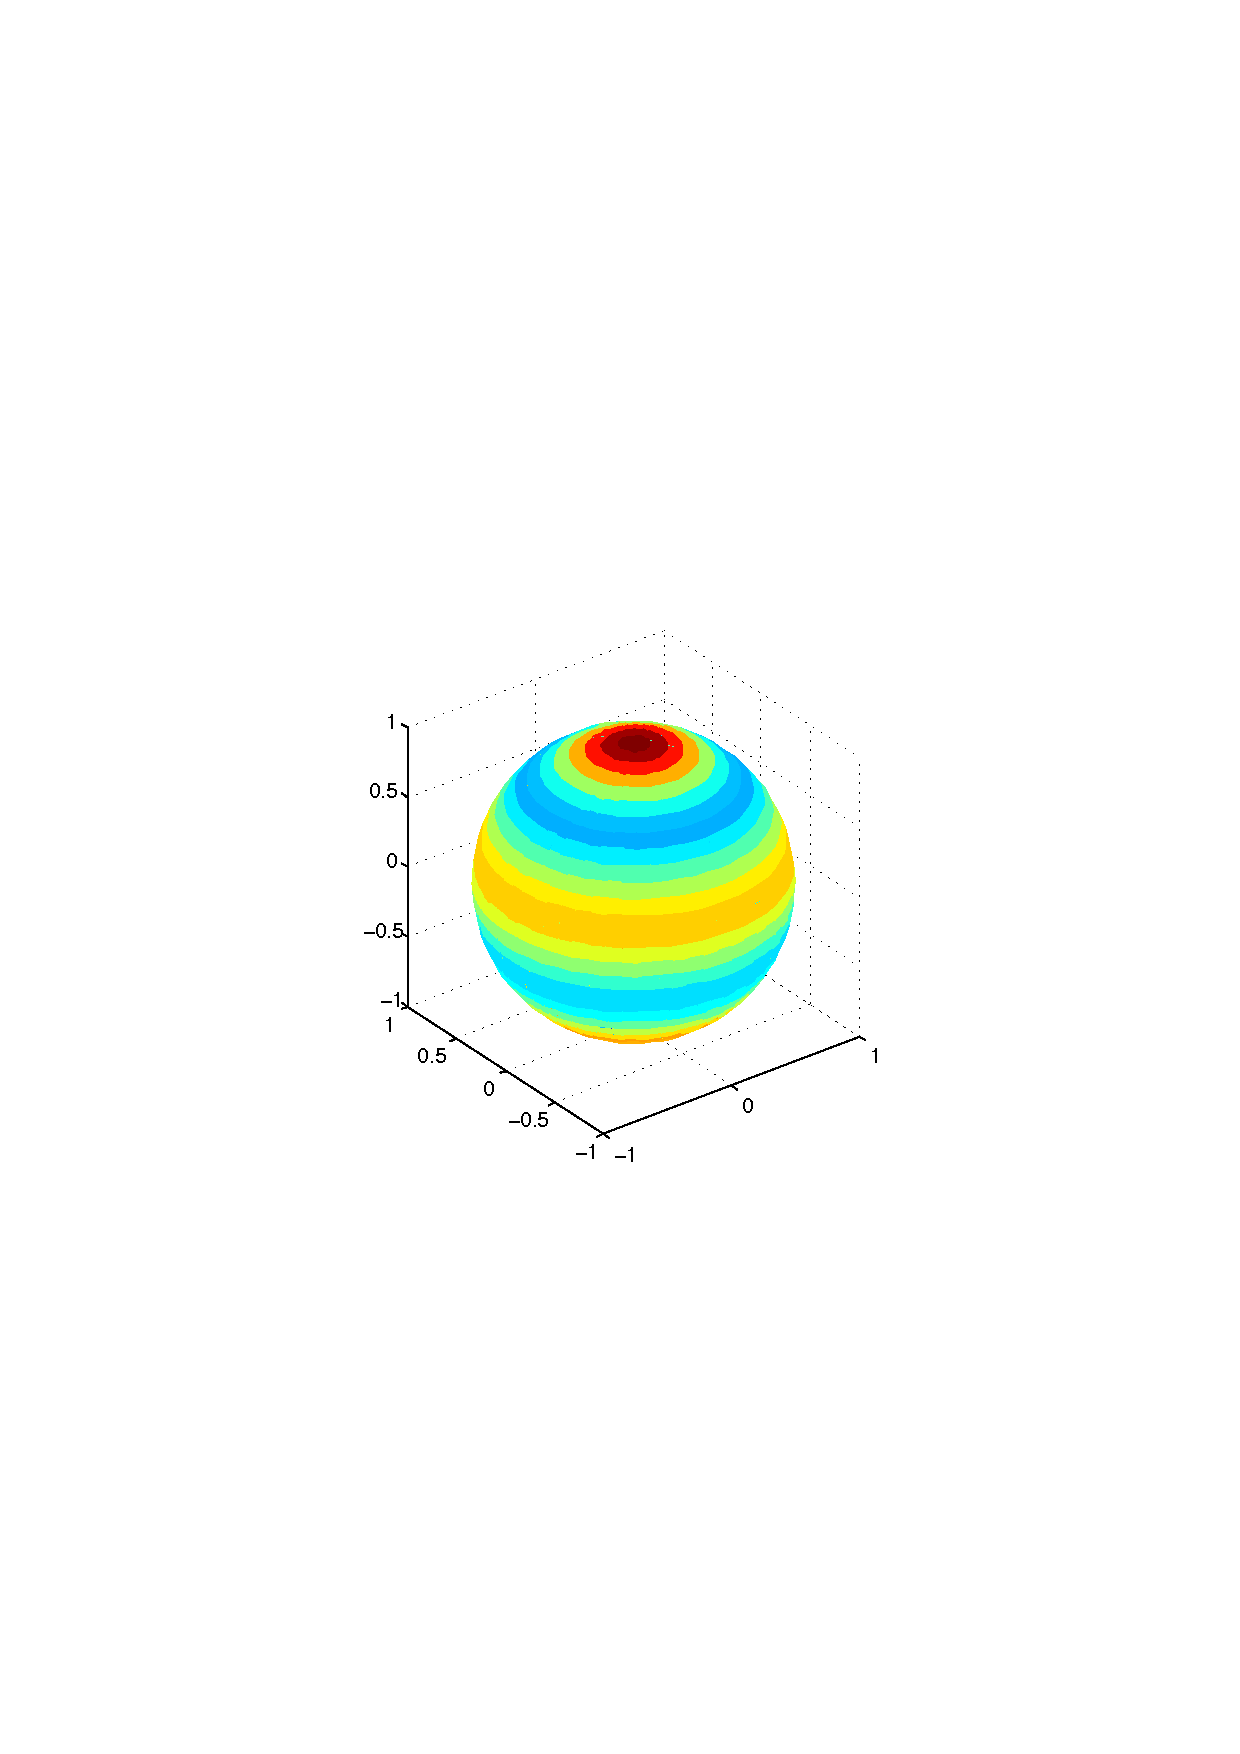
\includegraphics[width=0.45\textwidth]{kugel/ylm/a_5_0.pdf}
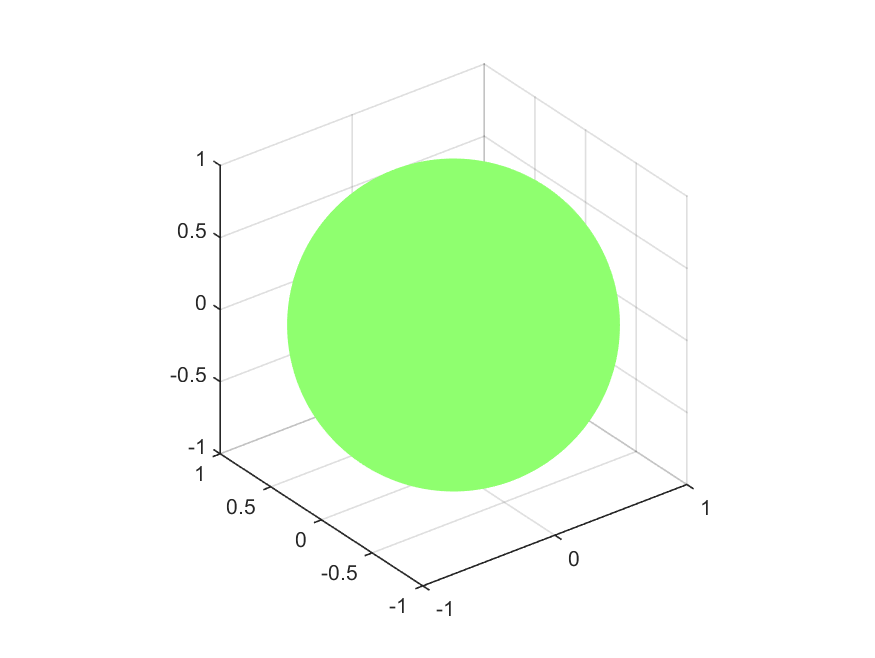
\includegraphics[width=0.45\textwidth]{kugel/ylm/b_5_0.pdf}
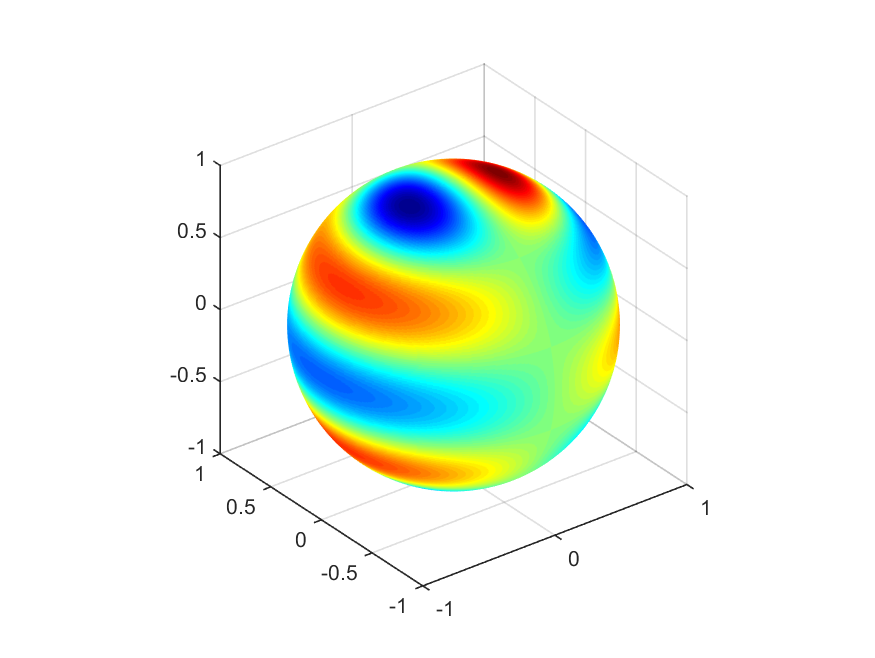
\includegraphics[width=0.45\textwidth]{kugel/ylm/a_5_1.pdf}
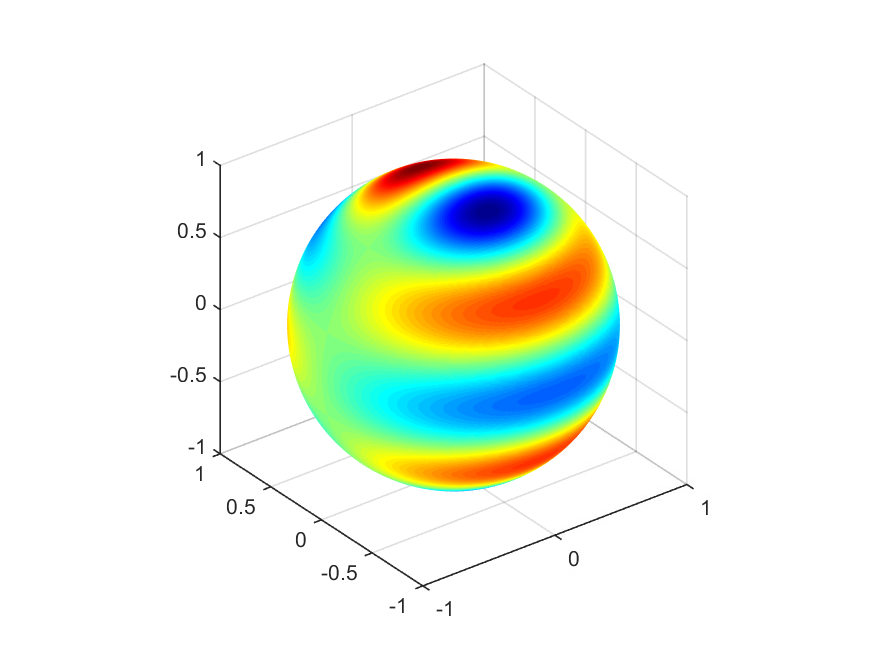
\includegraphics[width=0.45\textwidth]{kugel/ylm/b_5_1.pdf}
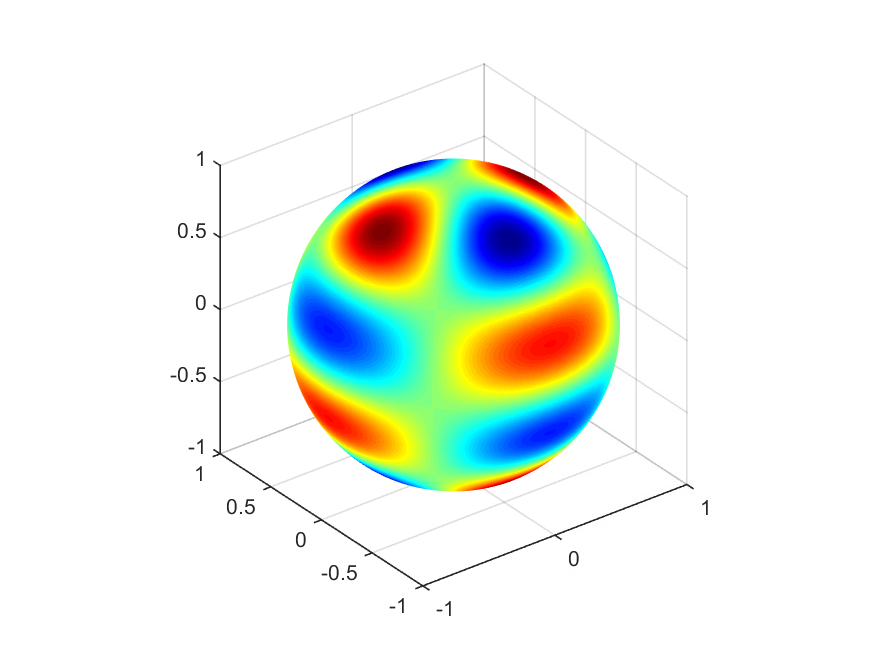
\includegraphics[width=0.45\textwidth]{kugel/ylm/a_5_2.pdf}
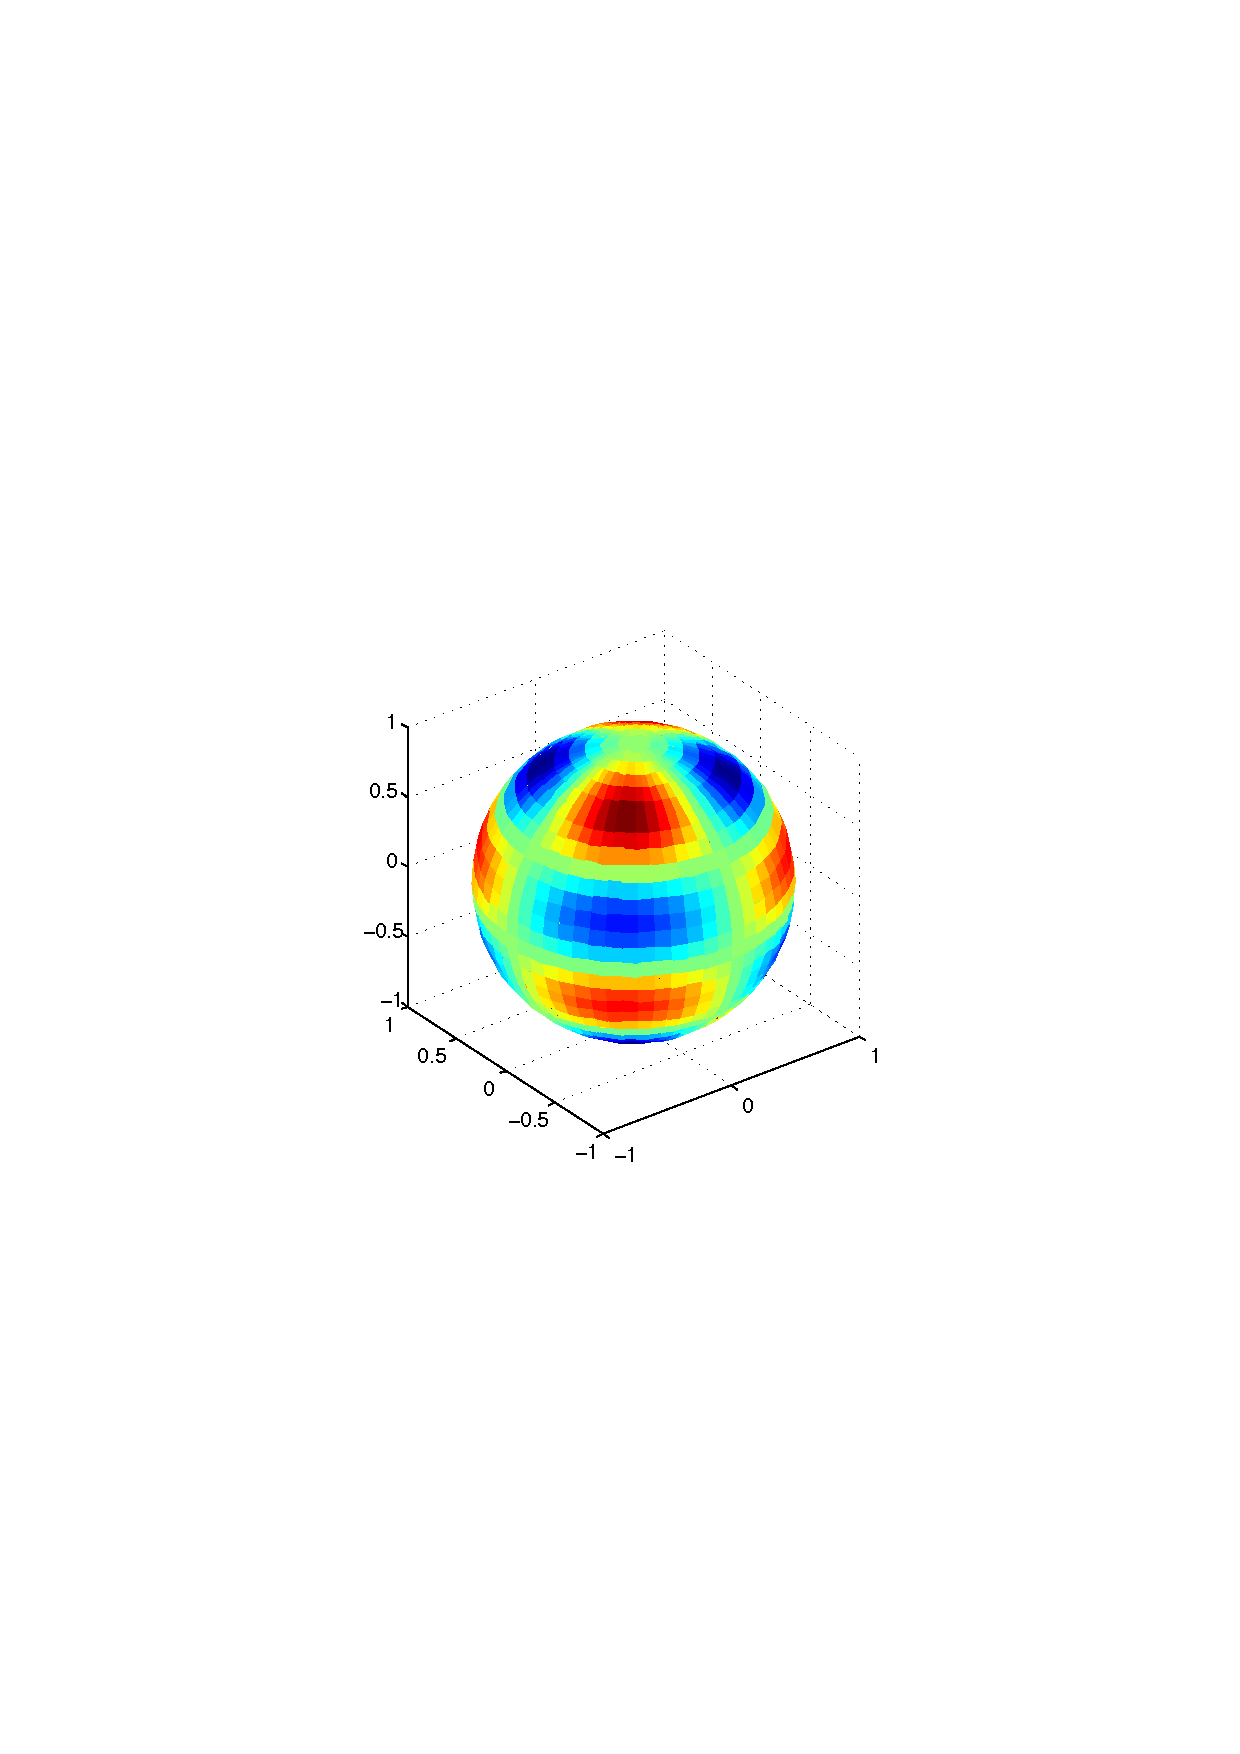
\includegraphics[width=0.45\textwidth]{kugel/ylm/b_5_2.pdf}
\caption{$Y_{lm}$ mit $l=5$, $m=0$, 1, 2 $\&$ $Z_{lm}$ mit $l=5$, $m=0$, 1, 2
\label{skript:Bild 0}}
\end{figure}

\begin{figure}% Bilder 3-5 Y_lm und Z_lm
\centering
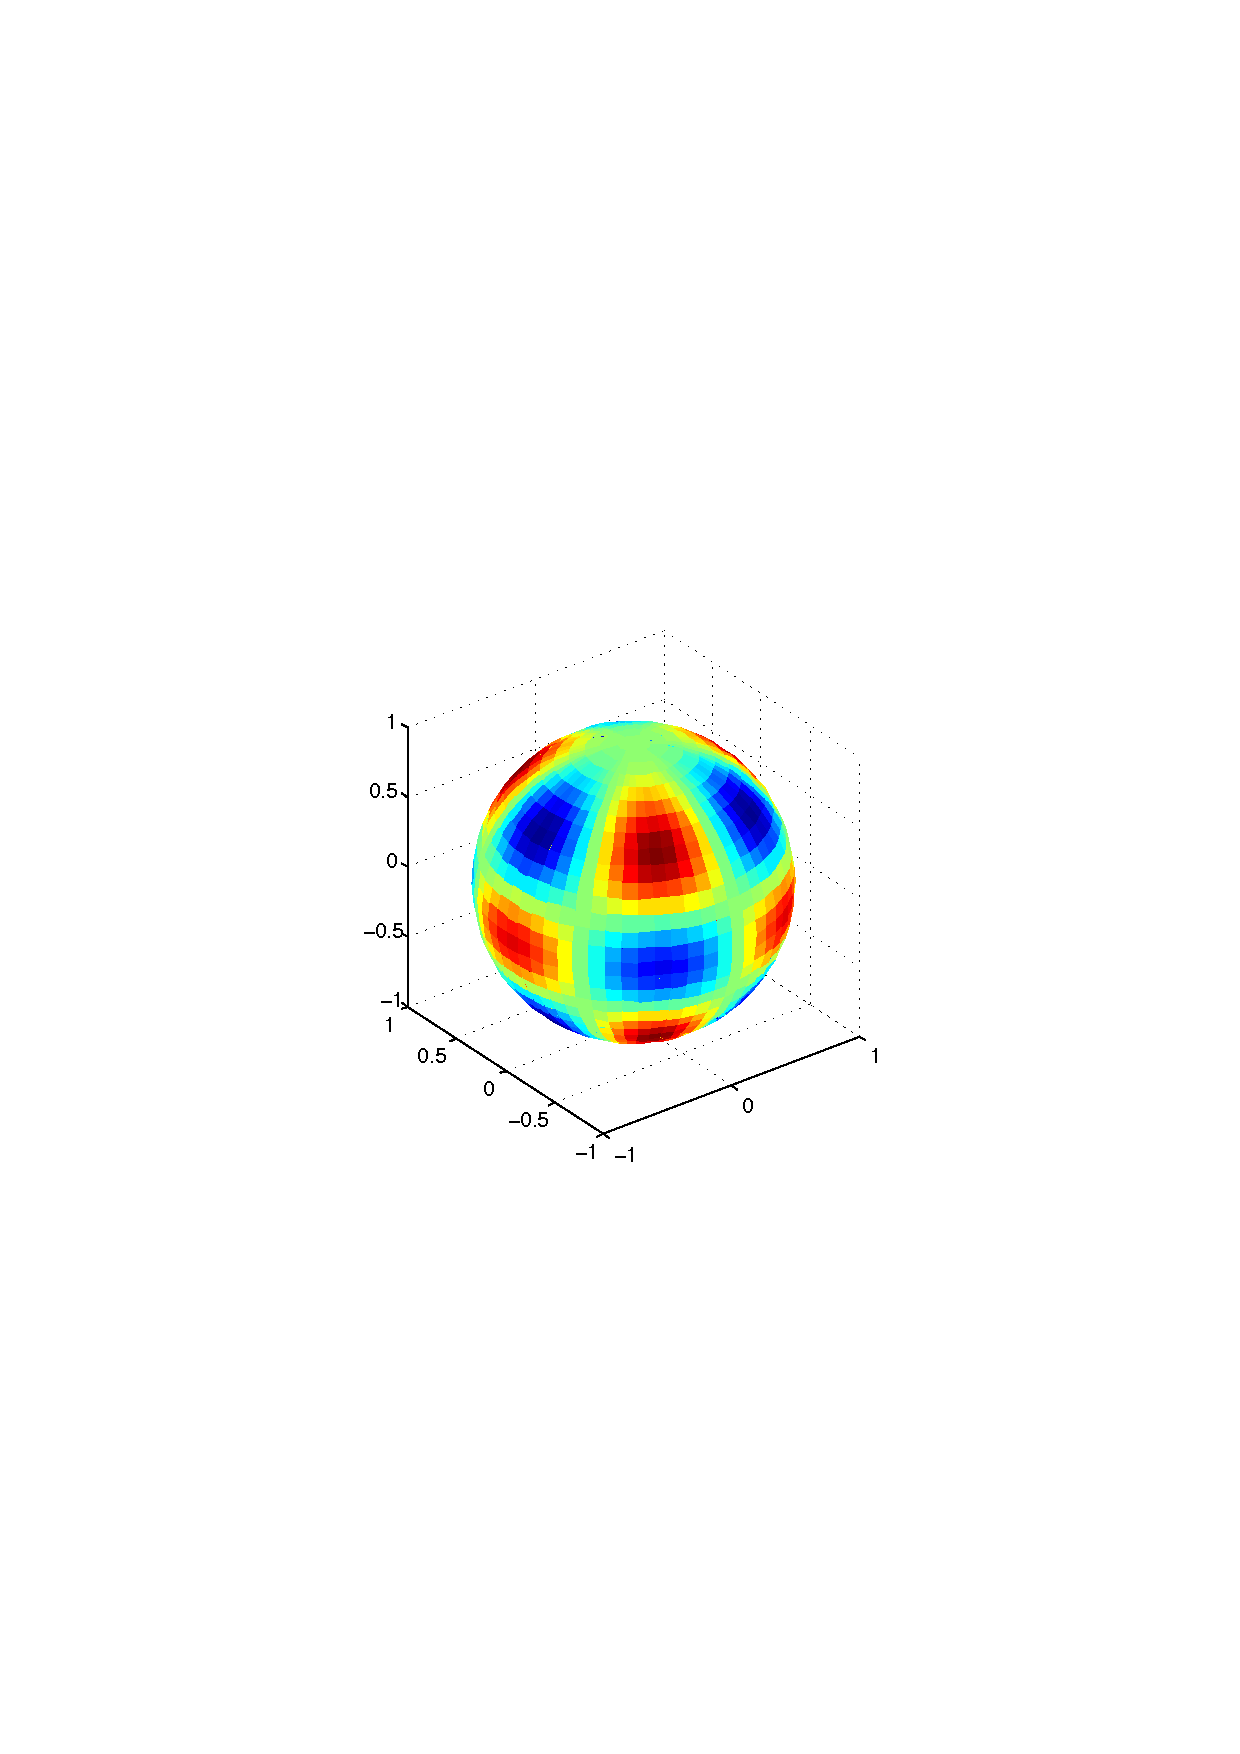
\includegraphics[width=0.45\textwidth]{kugel/ylm/a_5_3.pdf}
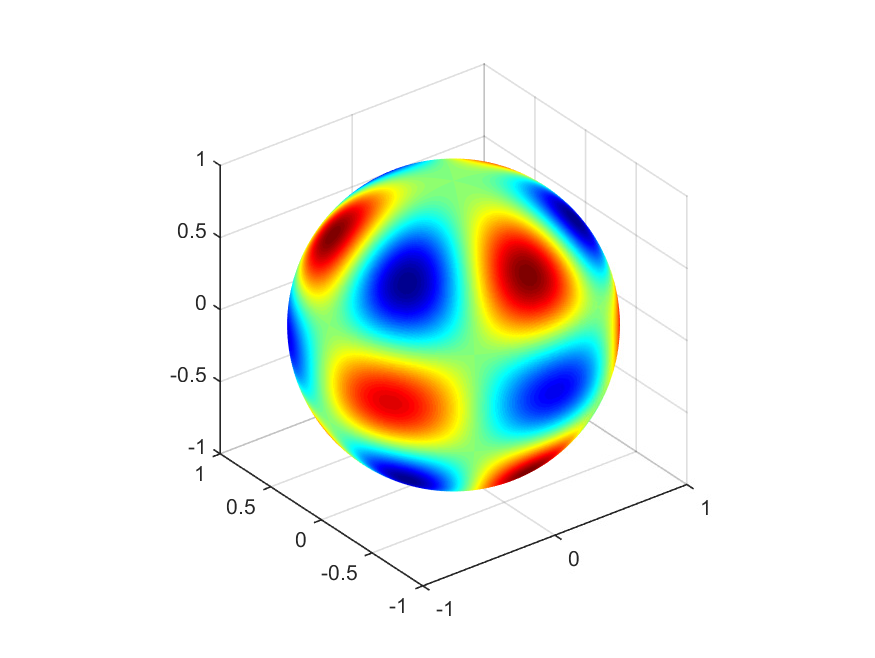
\includegraphics[width=0.45\textwidth]{kugel/ylm/b_5_3.pdf}
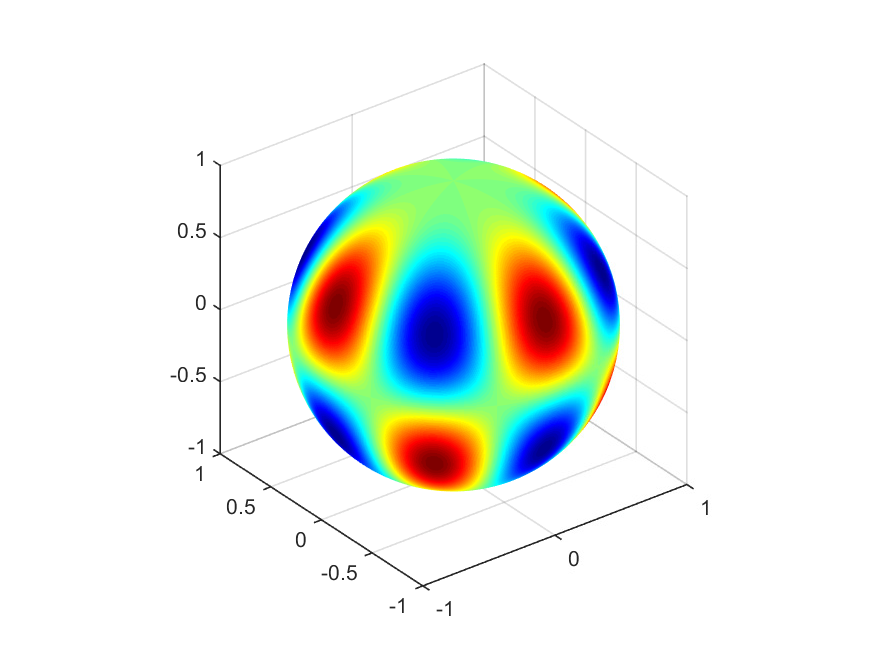
\includegraphics[width=0.45\textwidth]{kugel/ylm/a_5_4.pdf}
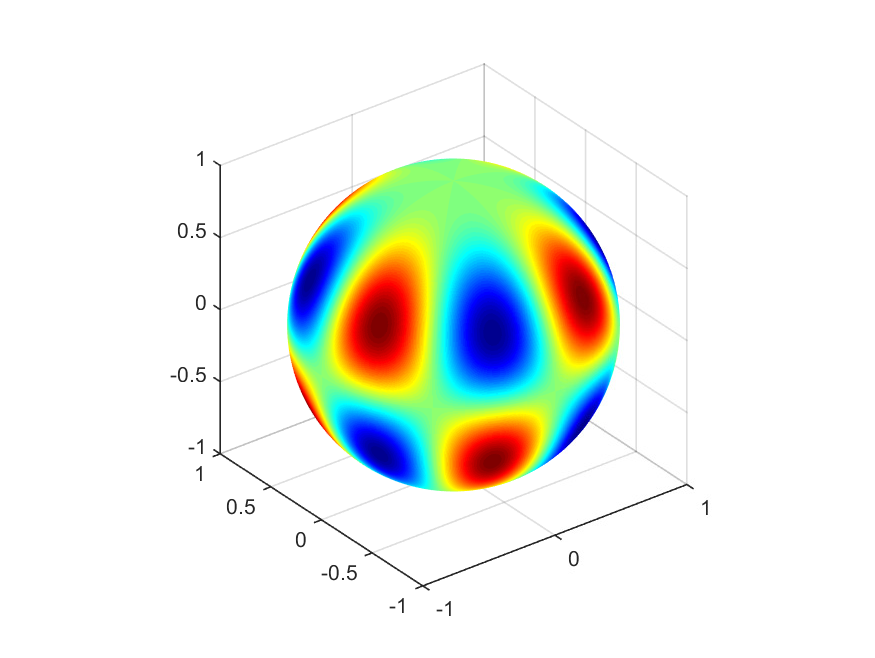
\includegraphics[width=0.45\textwidth]{kugel/ylm/b_5_4.pdf}
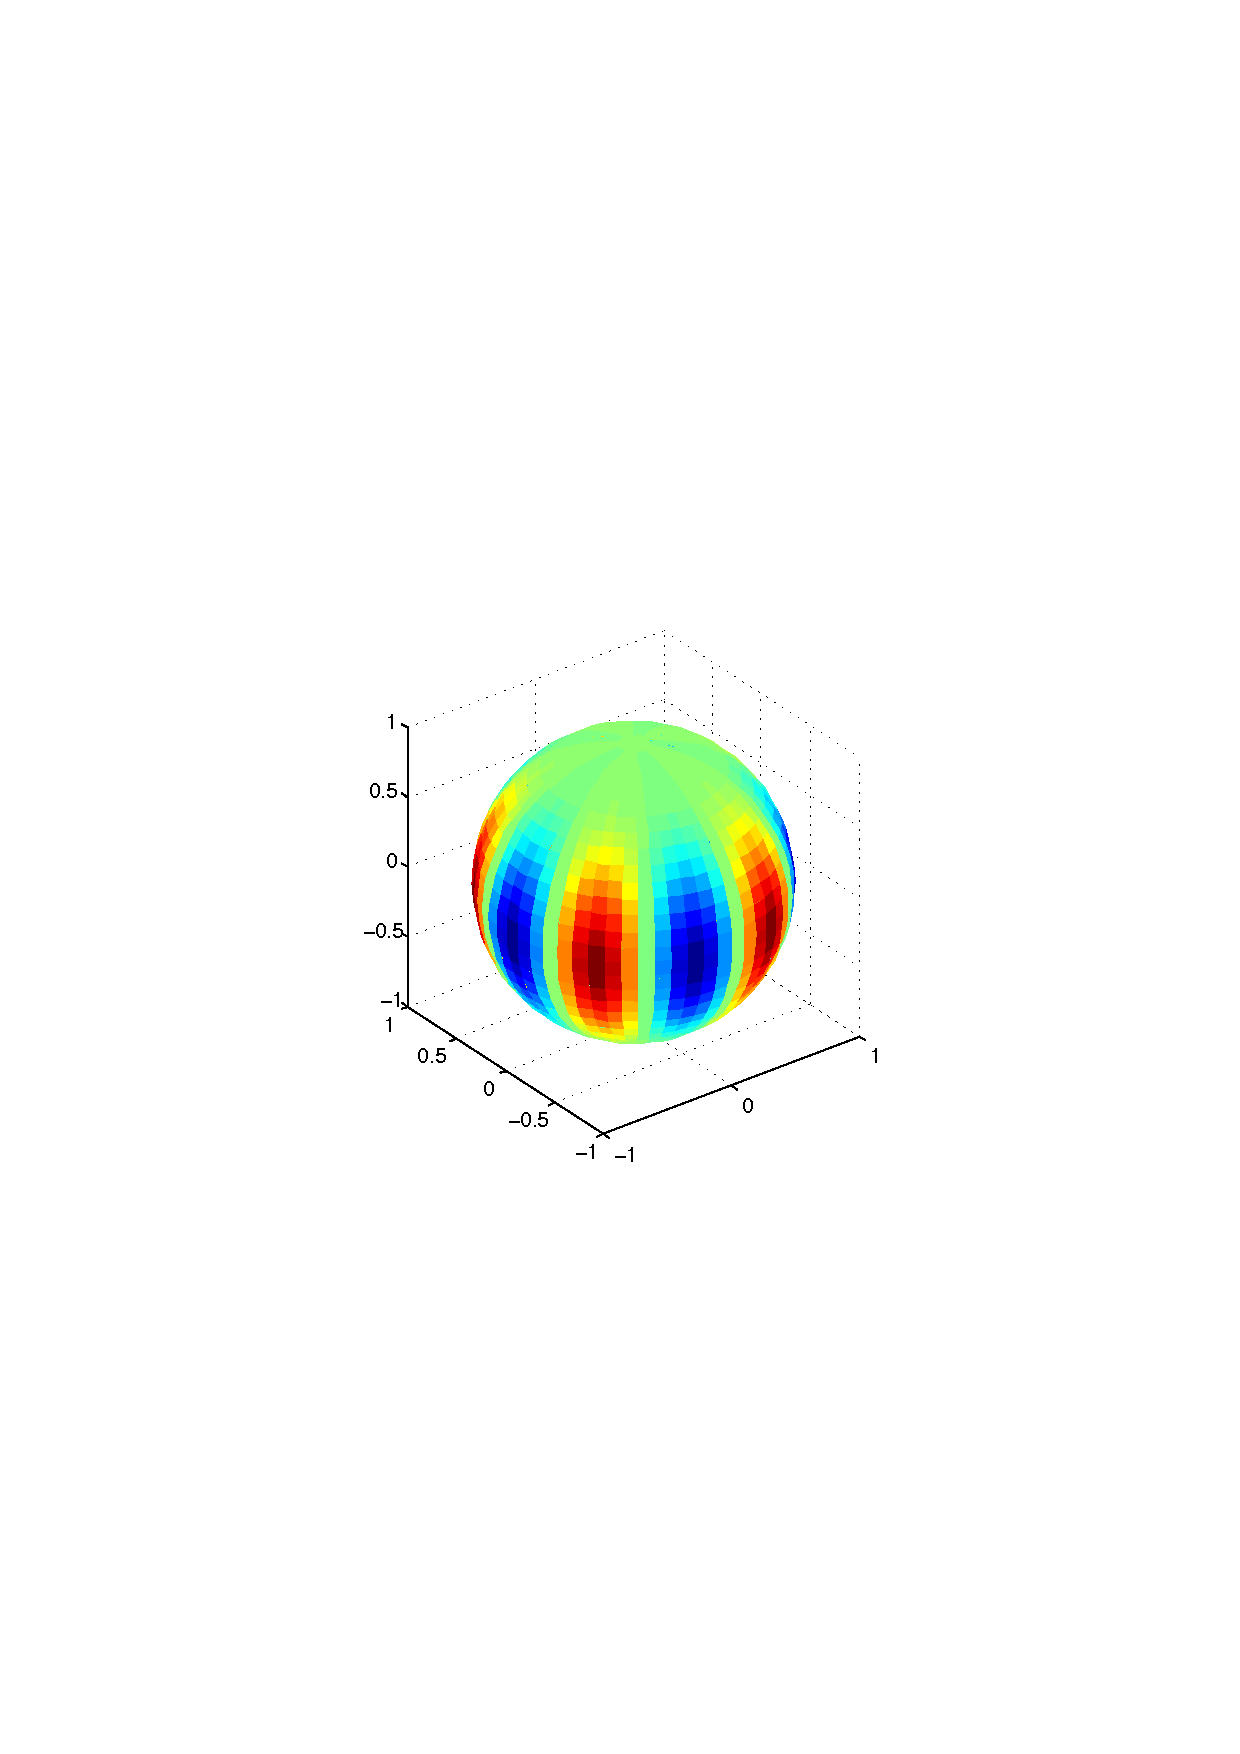
\includegraphics[width=0.45\textwidth]{kugel/ylm/a_5_5.pdf}
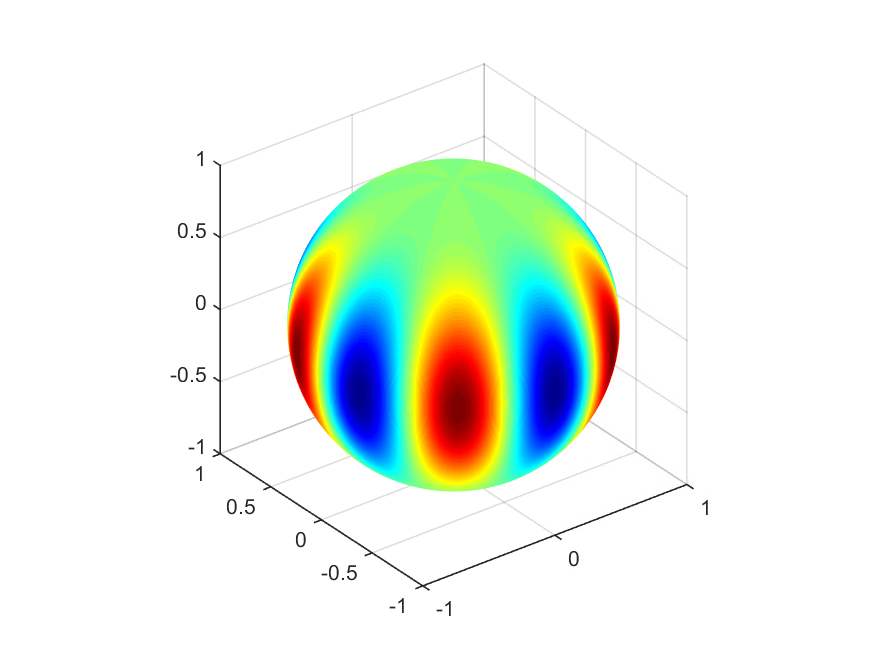
\includegraphics[width=0.45\textwidth]{kugel/ylm/b_5_5.pdf}
\caption{$Y_{lm}$ mit $l=5$, $m=3$, 4, 5 $\&$ $Z_{lm}$ mit $l=5$, $m=3$, 4, 5
\label{skript:Bild 2}}
\end{figure}

\subsection{Fourier-Koeffizienten}
Die Berechnung der Fourier-Koeffizienten in der klassischen 
Fourier-Theorie erfolgt folgendermassen:
\begin{align*}
k&= 0: & a_{0} &= \frac{1}{2\pi} \int_{-\pi}^\pi f(x) \cdot dx
\\
&  & b_{0} &= 0
\\
k& > 0: & a_{k} &= \frac{1}{\pi} \int_{-\pi}^\pi f(x) \cdot \cos kx \cdot dx
\\
& & b_{k} &= \frac{1}{\pi} \int_{-\pi}^\pi f(x) \cdot \sin kx \cdot dx
\end{align*}
F"ur die Berechnung der Fourier-Koeffizienten auf der Kugeloberfl"ache 
verwendet man folgende Formeln:
\begin{align*}
l&=0: & a_{00} &= \frac{1}{4\pi} \int_{-\pi}^\pi \int_{0}^\pi f(\vartheta,\varphi) \cdot \sin\vartheta \cdot d\vartheta \cdot d\varphi
\\
&  & b_{00} &= 0
\\
l&\ne 0: & a_{lm} &= \frac{1}{4\pi} \int_{-\pi}^\pi \int_{0}^\pi f(\vartheta,\varphi) \cdot Y_{lm} (\vartheta, \varphi) \cdot \sin\vartheta \cdot d\vartheta \cdot d\varphi
\\
&  & b_{lm} &= \frac{1}{4\pi} \int_{-\pi}^\pi \int_{0}^\pi f(\vartheta,\varphi) \cdot Z_{lm} (\vartheta, \varphi) \cdot \sin\vartheta \cdot d\vartheta \cdot d\varphi
\end{align*}

\subsection{Berechnung der Funktion aus den Fourier-Koeffizienten}
Um eine Funktion wieder zu rekonstruieren, muss man die einzelnen 
Wellenfunktionen, gewichten mit den entsprechenden Fourier-Koeffizienten 
wieder aufsummieren.
In der klassischen Fourier-Theorie wird folgendermassen vorgegangen:
\begin{align*}
f(x)&=a_0 + \sum_{n=0}^\infty a_k \cdot \cos kx + b_k \sin kx
\end{align*}
Will man eine Funktion auf der Kugeloberfl"ache wieder rekonstruieren, 
muss man folgende Formel verwenden:
\begin{align*}
f(\vartheta, \varphi) &= a_{00} + \sum_{l=1}^\infty \sum_{m=0}^l a_{lm} \cdot Y_{lm} + b_{lm} \cdot Z_{lm}
\end{align*}

\subsection{Kugelspektrum}
Um das komplexe Amplitudenspektrum darstellen zu k"onnen, muss man die
Sinus- und Kosinus-Koeffizienten noch folgendermassen zusammenfassen:
\begin{align*}
c_k= \sqrt{a^2_{k}+b^2_{k}}
\end{align*}
Analog zum komplexen Amplitudenspektrum kann man ein Kugelspektrum 
darstellen. 
Die Zusammenfassung der Koeffizienten erfolgt in dem Fall mittels 
dieser Formel:
\begin{align*}
c_l=\sum_{m=0}^l \sqrt{a^2_{lm}+b^2_{lm}}
\end{align*}

\subsection{Nummerische Berechnung des Kugelspektrum}
Allf"allige Abweichungen in unseren Darstellungen sind auf die 
numerischen Berechnungen zur"uckzuf"uhren, da wir 
$d\vartheta$ und $d\varphi$ nicht beliebig klein w"ahlen konnten.
Qualitativ sind jedoch alle Ergebnisse korrekt.

\section{Spektrum einer Rechteckfunktion}
\rhead{Spektrum einer Rechteckfunktion}
In der nachfolgenden Bilderreihe kann man sehen, dass egal wo ein 
Signal auftritt, das komplexe Amplitudenspektrum in jedem Fall gleich 
bleibt.

\begin{figure}
\centering
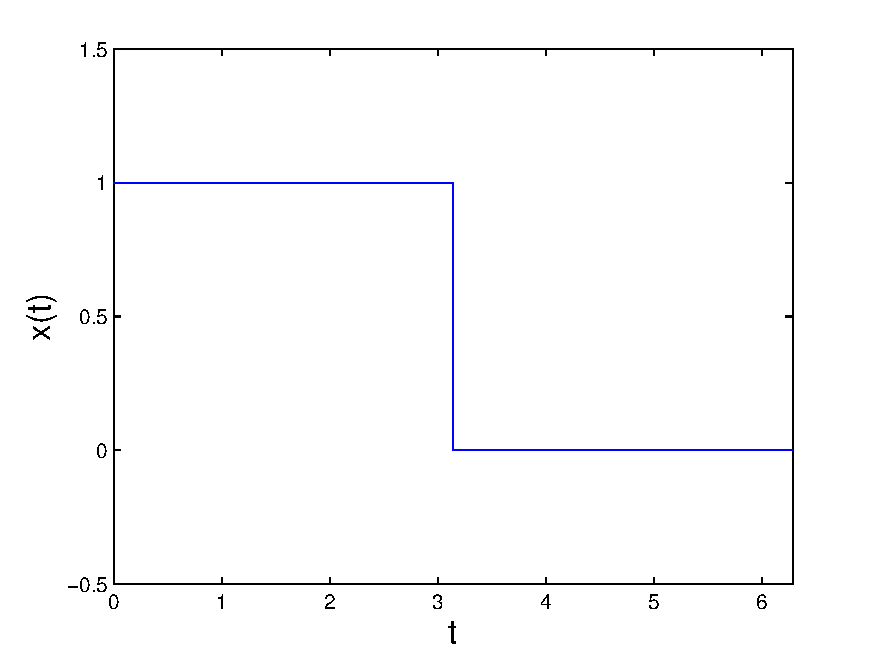
\includegraphics[width=0.45\textwidth]{kugel/kSpektrum/Rechteck1_1.pdf}
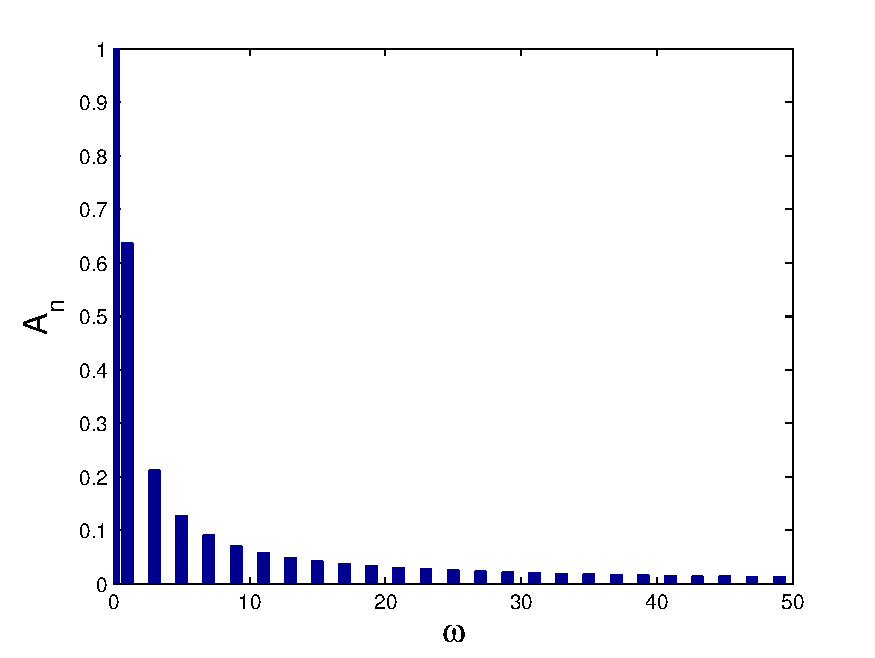
\includegraphics[width=0.45\textwidth]{kugel/kSpektrum/Rechteck1_2.pdf}
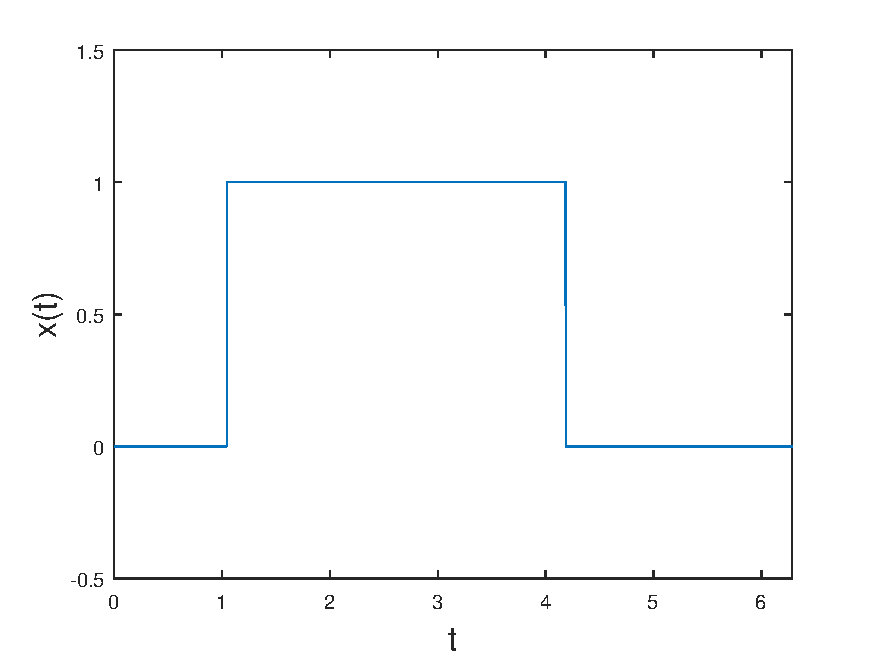
\includegraphics[width=0.45\textwidth]{kugel/kSpektrum/Rechteck2_1.pdf}
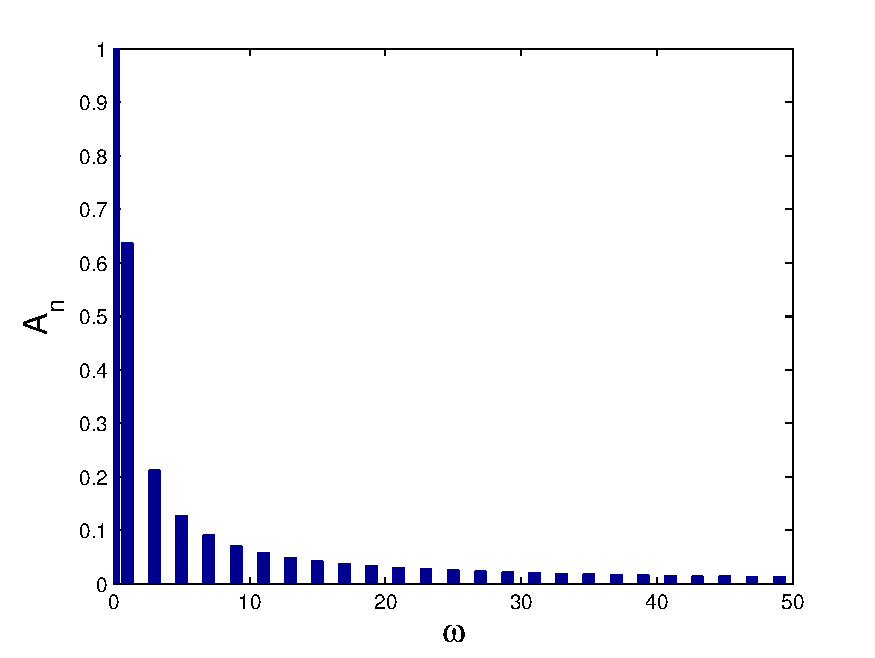
\includegraphics[width=0.45\textwidth]{kugel/kSpektrum/Rechteck1_2.pdf}
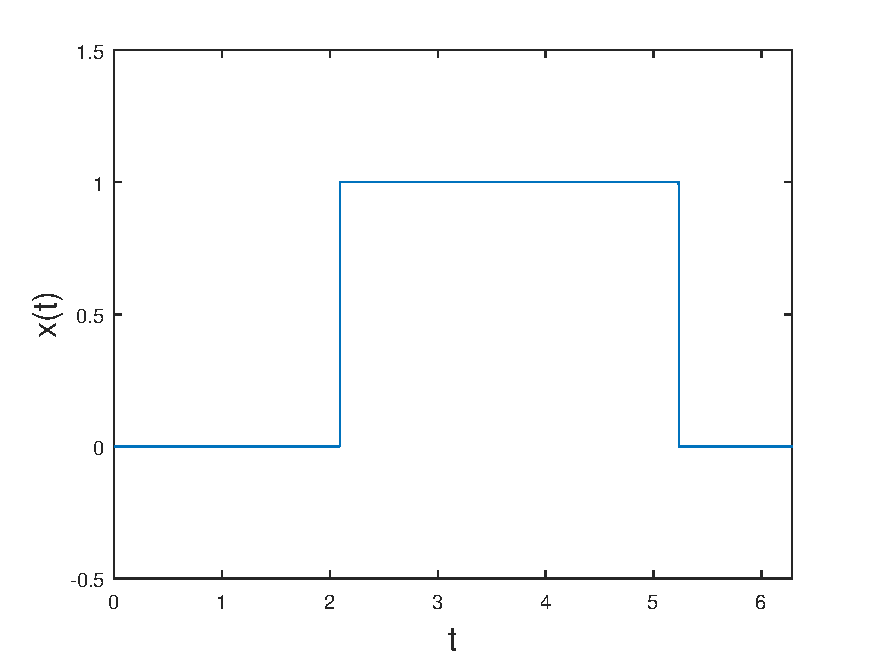
\includegraphics[width=0.45\textwidth]{kugel/kSpektrum/Rechteck3_1.pdf}
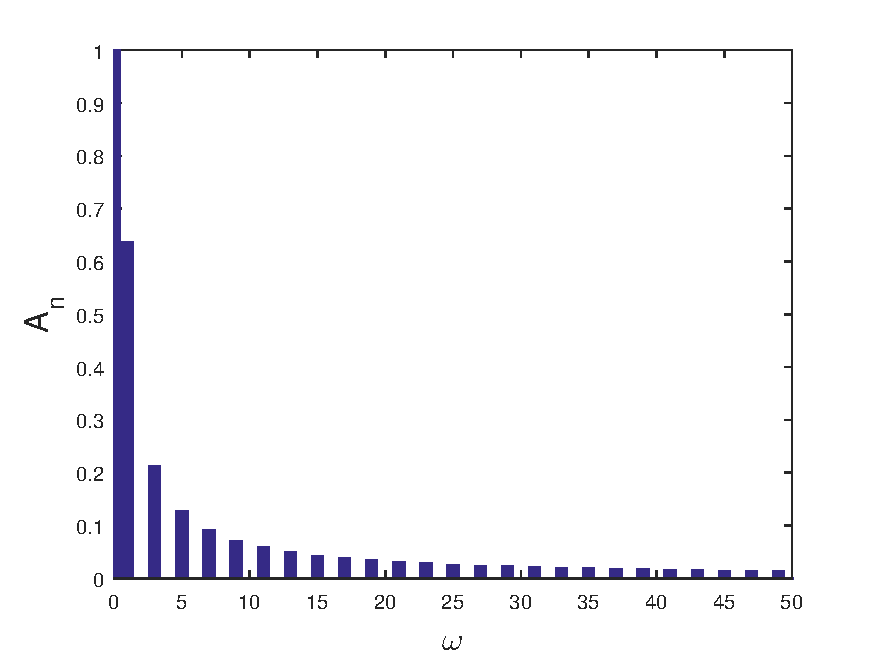
\includegraphics[width=0.45\textwidth]{kugel/kSpektrum/Rechteck3_2.pdf}
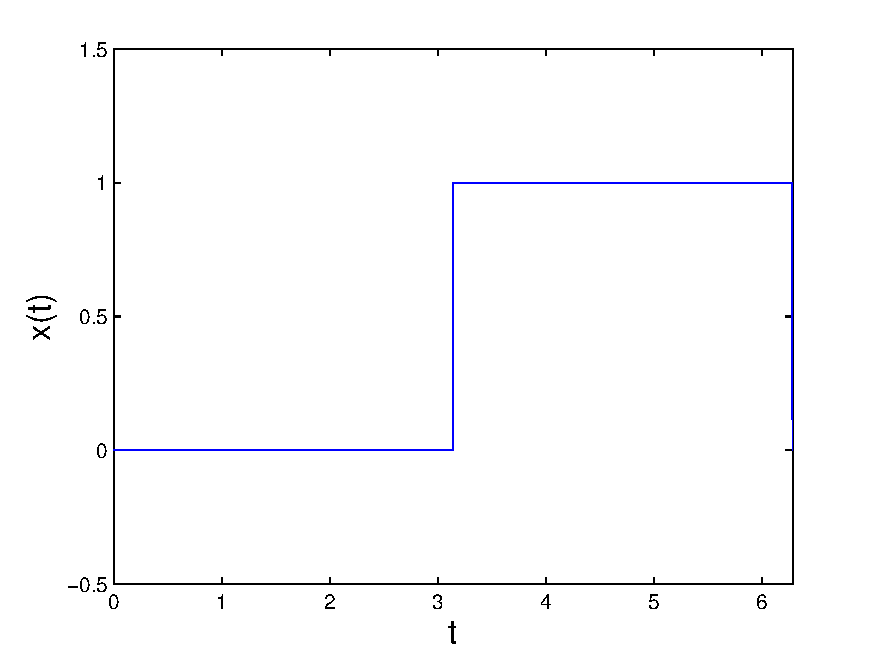
\includegraphics[width=0.45\textwidth]{kugel/kSpektrum/Rechteck4_1.pdf}
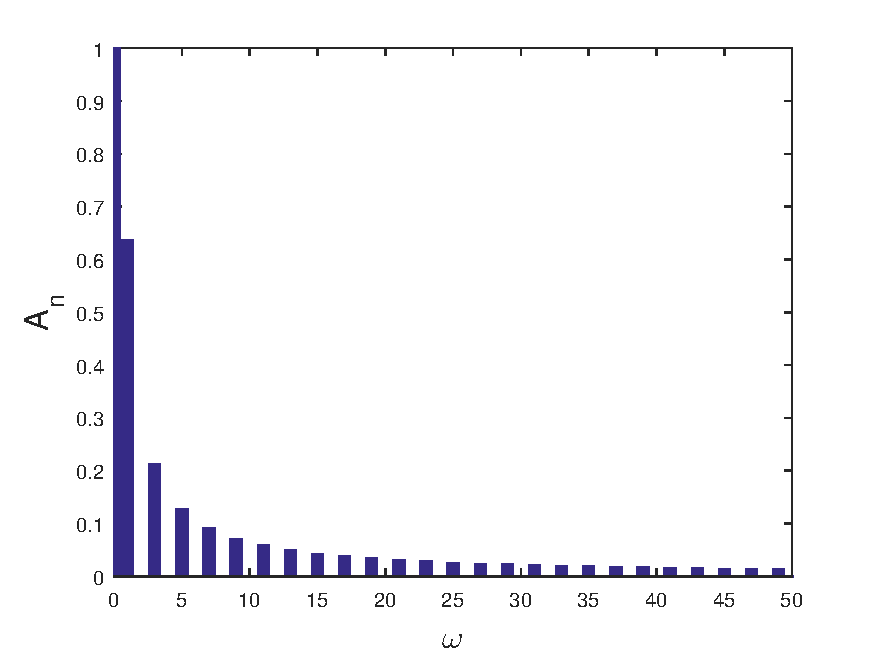
\includegraphics[width=0.45\textwidth]{kugel/kSpektrum/Rechteck4_2.pdf}
%\caption{Titel??
\label{skript:Spektrum1}%}
\end{figure}
Dasselbe gilt auch f"ur Funktionen auf der Kugeloberfl"ache, wie man
auf den folgenden Bildern sehen kann.
\begin{figure}
\centering
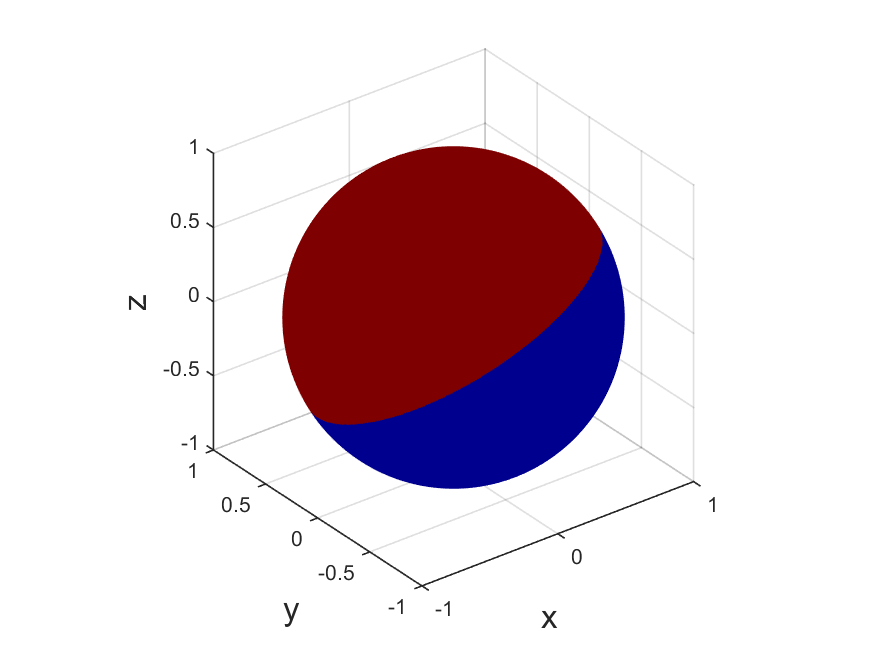
\includegraphics[width=0.45\textwidth]{kugel/kSpektrum/Kugel_1_1.pdf}
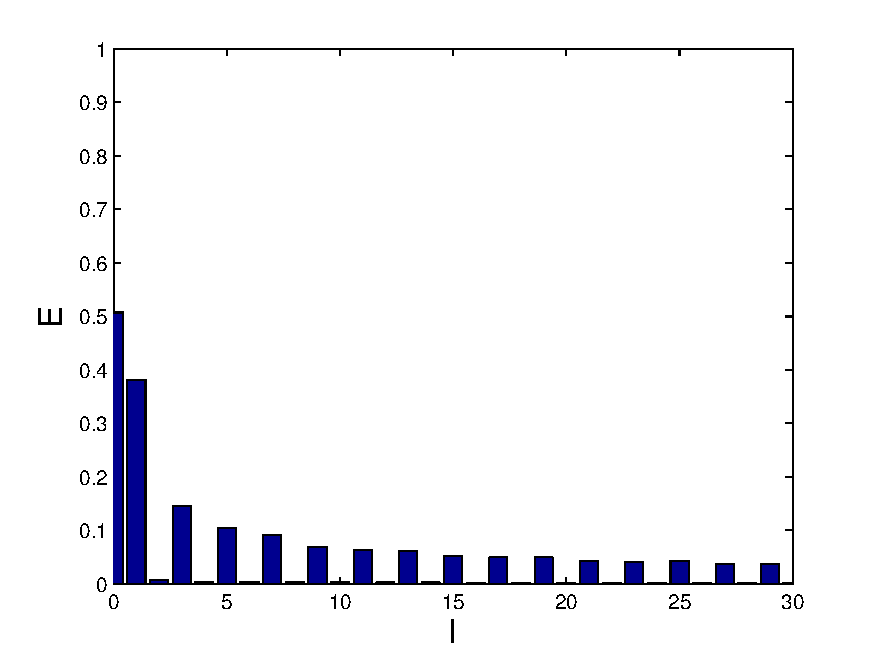
\includegraphics[width=0.45\textwidth]{kugel/kSpektrum/Kugel_1_2.pdf}
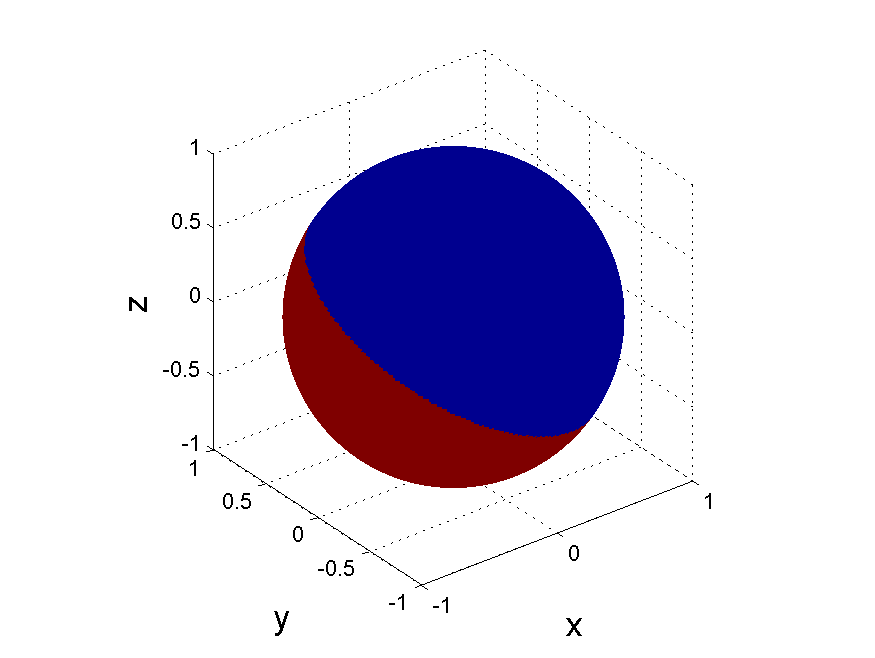
\includegraphics[width=0.45\textwidth]{kugel/kSpektrum/Kugel_2_1.pdf}
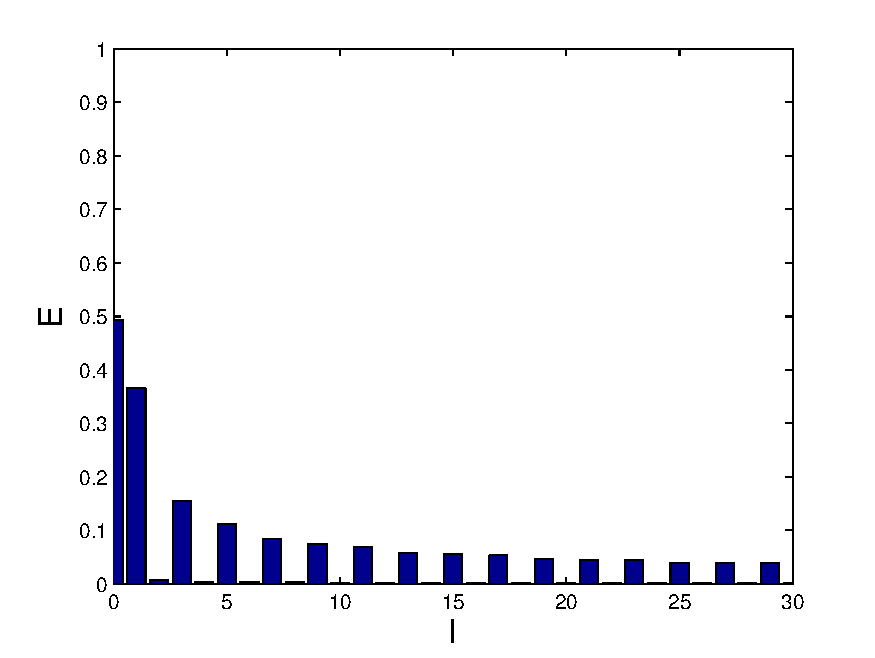
\includegraphics[width=0.45\textwidth]{kugel/kSpektrum/Kugel_2_2.pdf}
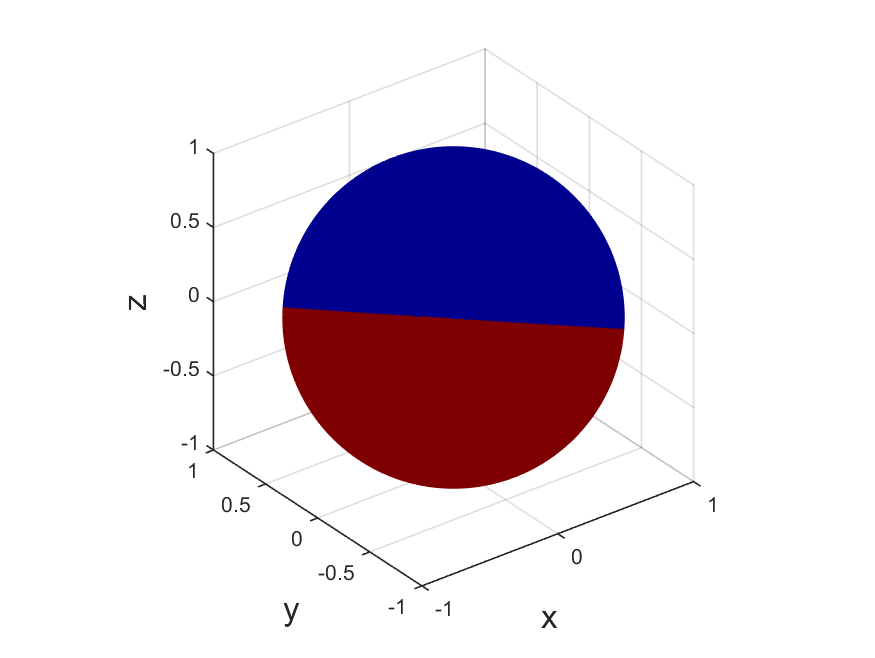
\includegraphics[width=0.45\textwidth]{kugel/kSpektrum/Kugel_3_1.pdf}
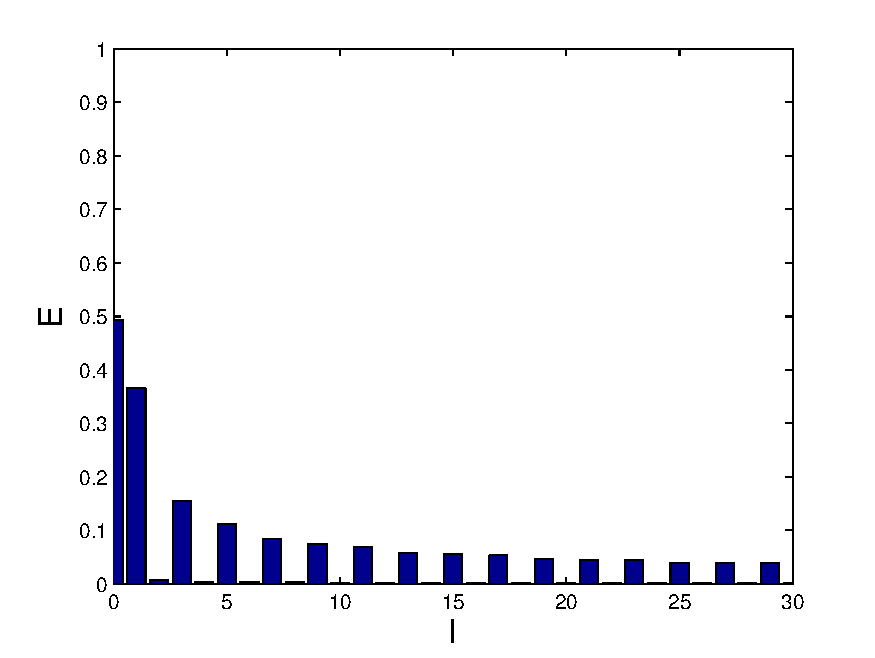
\includegraphics[width=0.45\textwidth]{kugel/kSpektrum/Kugel_3_2.pdf}
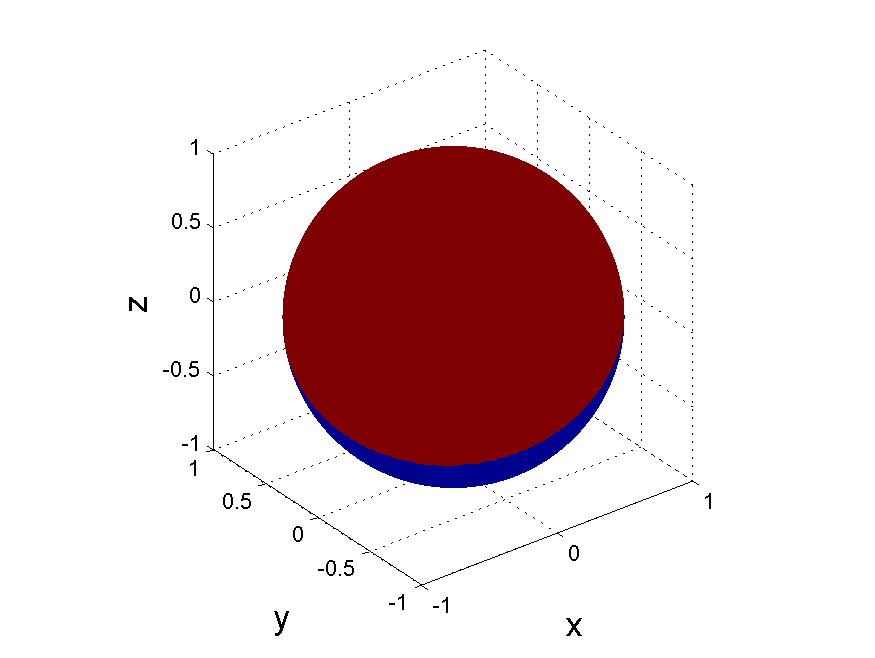
\includegraphics[width=0.45\textwidth]{kugel/kSpektrum/Kugel_4_1.pdf}
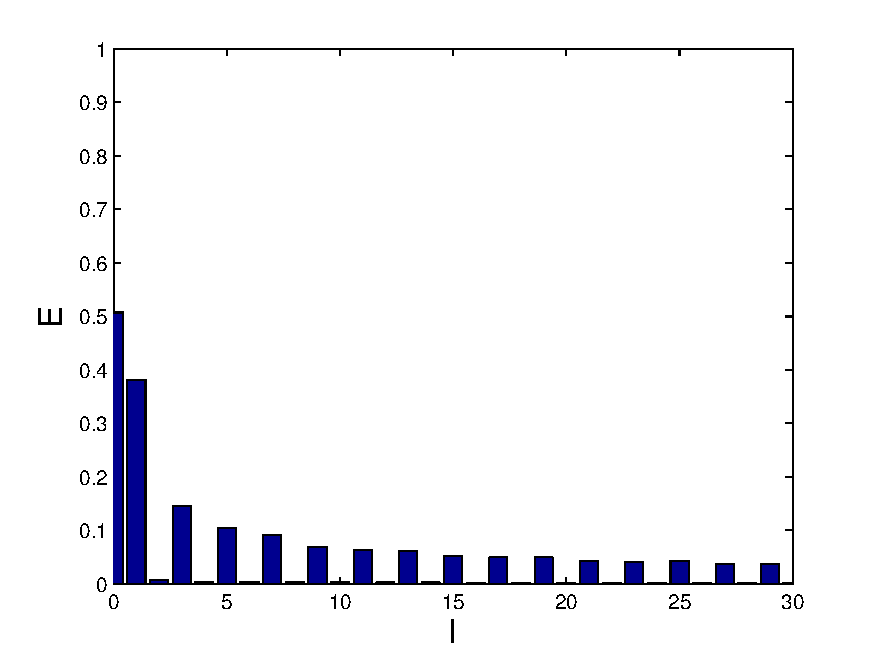
\includegraphics[width=0.45\textwidth]{kugel/kSpektrum/Kugel_4_2.pdf}
%\caption{Titel??
\label{skript:Spektrum1}%}
\end{figure}

\section{Dirac Stoss und konstante Funktion}
\rhead{Dirac Stoss und konstante Funktion}

Die folgende Bilderreihe zeigt auf, dass im Fall von einem Dirac-Stoss
alle Frequenzen gleich stark vertreten sind. 
Hingegen im Fall einer konstanteb Funktion nur noch der 0-te 
Koeffizient Gewichtet ist.Dies kann man sowohl beim Rechtecksignal 
wie auch bei Funktionen auf der Kugeloberfl"ache erkennen.

\begin{figure}
\centering
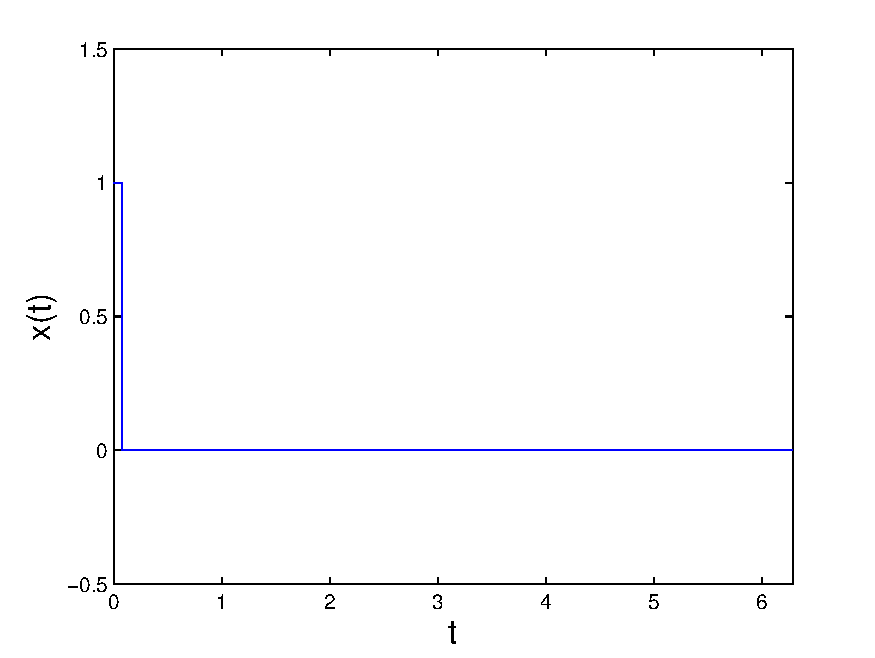
\includegraphics[width=0.45\textwidth]{kugel/Dkonstant/Rechteck1_1.pdf}
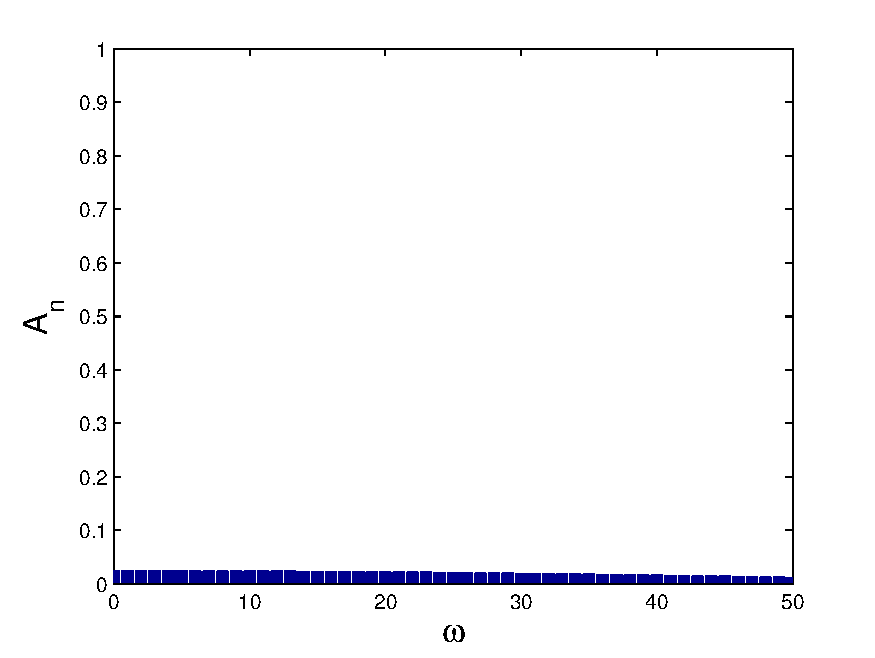
\includegraphics[width=0.45\textwidth]{kugel/Dkonstant/Rechteck1_2.pdf}
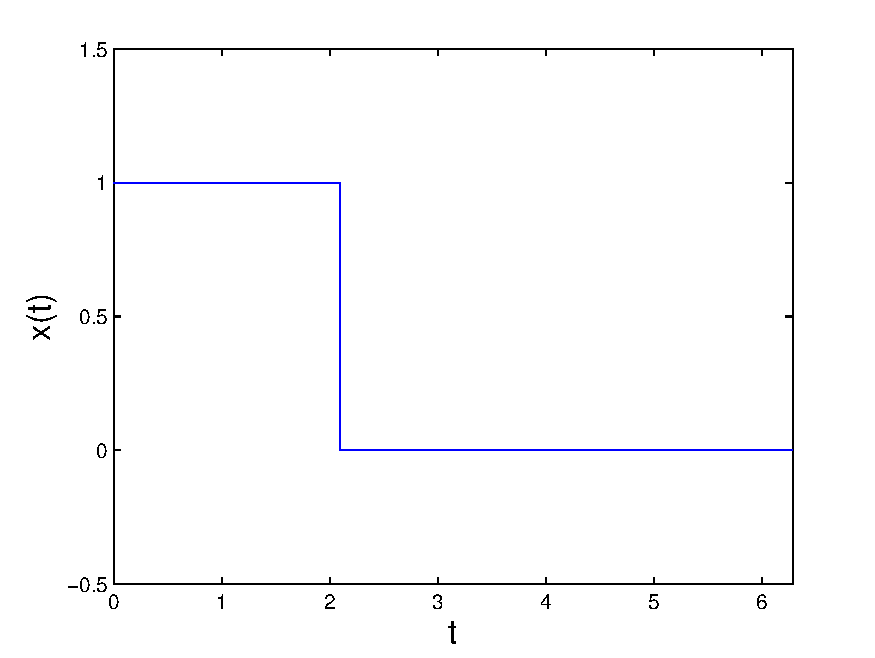
\includegraphics[width=0.45\textwidth]{kugel/Dkonstant/Rechteck2_1.pdf}
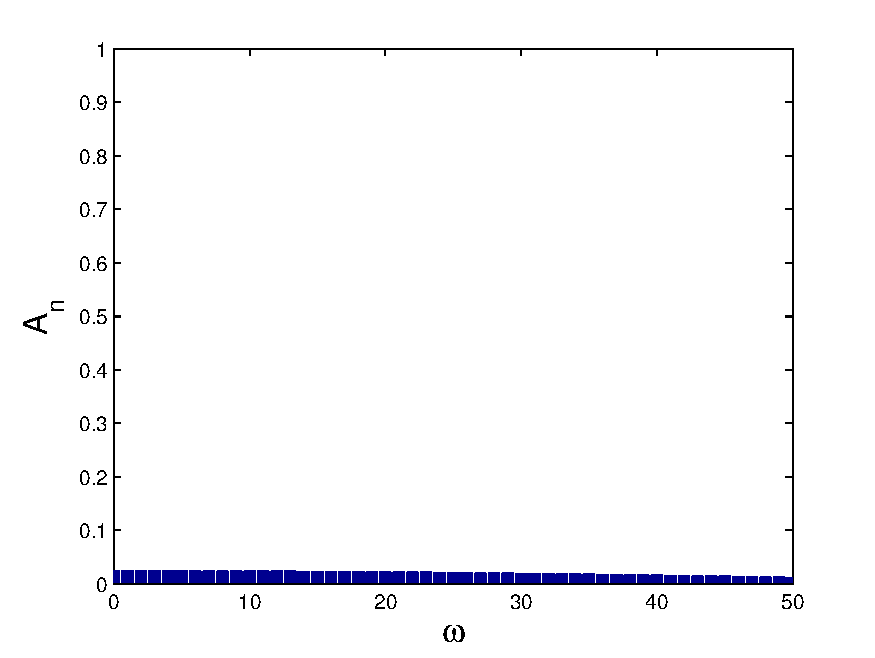
\includegraphics[width=0.45\textwidth]{kugel/Dkonstant/Rechteck1_2.pdf}
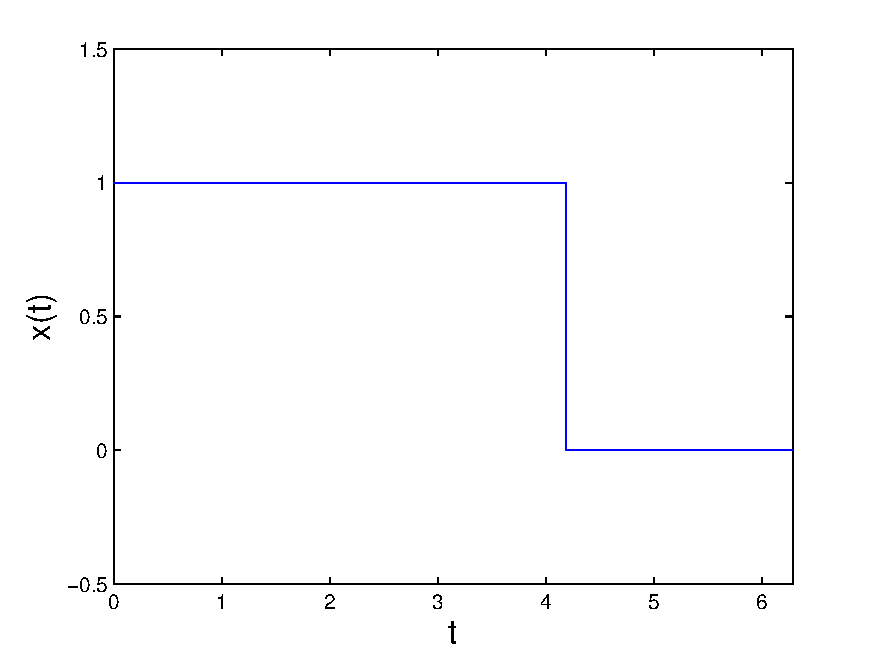
\includegraphics[width=0.45\textwidth]{kugel/Dkonstant/Rechteck3_1.pdf}
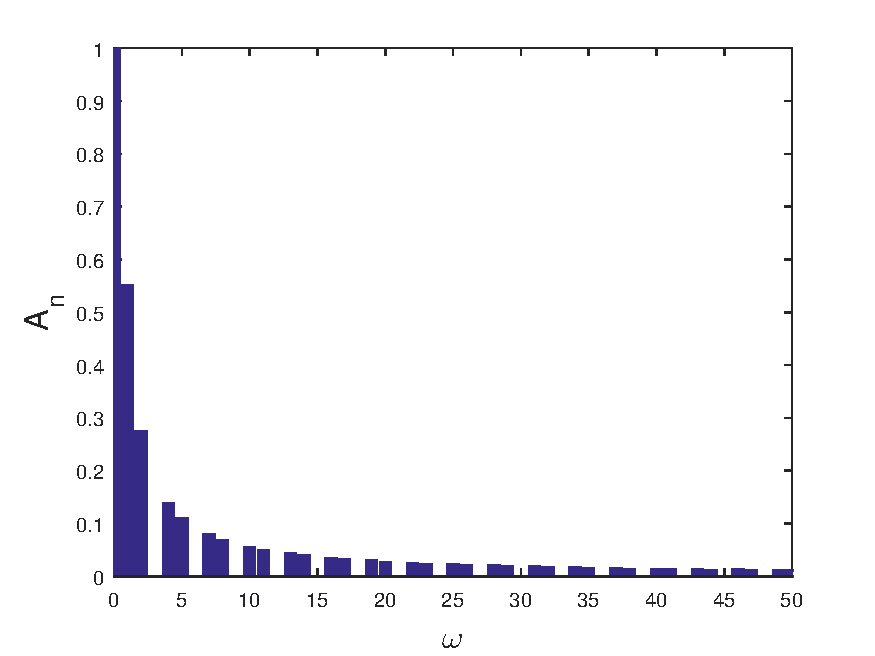
\includegraphics[width=0.45\textwidth]{kugel/Dkonstant/Rechteck3_2.pdf}
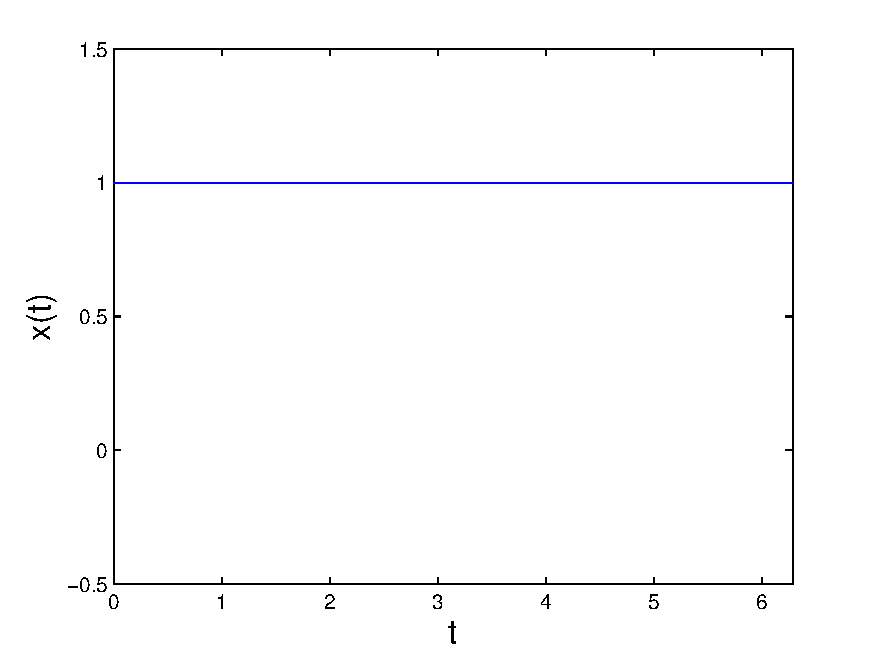
\includegraphics[width=0.45\textwidth]{kugel/Dkonstant/Rechteck4_1.pdf}
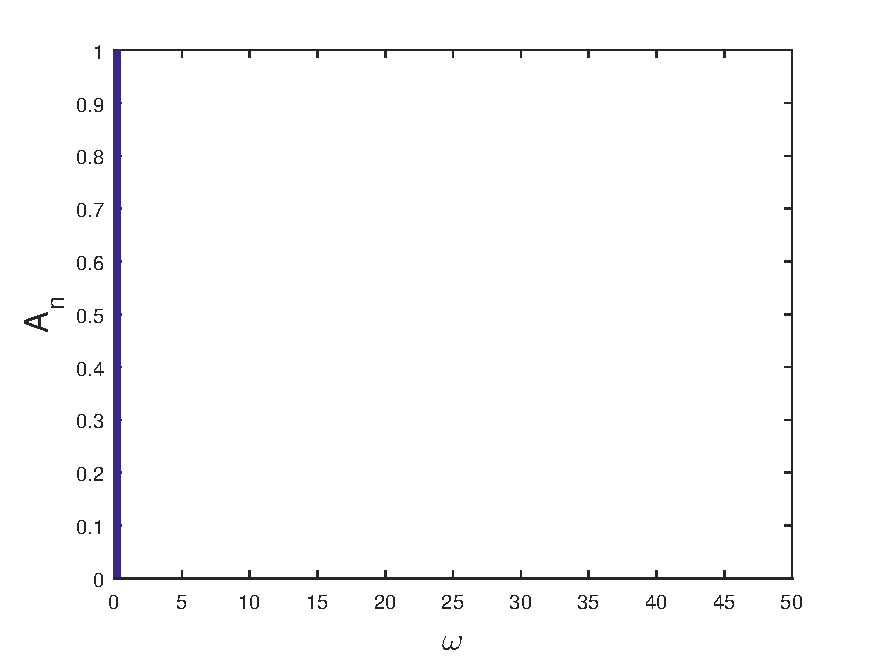
\includegraphics[width=0.45\textwidth]{kugel/Dkonstant/Rechteck4_2.pdf}
%\caption{Titel??
\label{skript:Dirac2}%}
\end{figure}

\begin{figure}
\centering
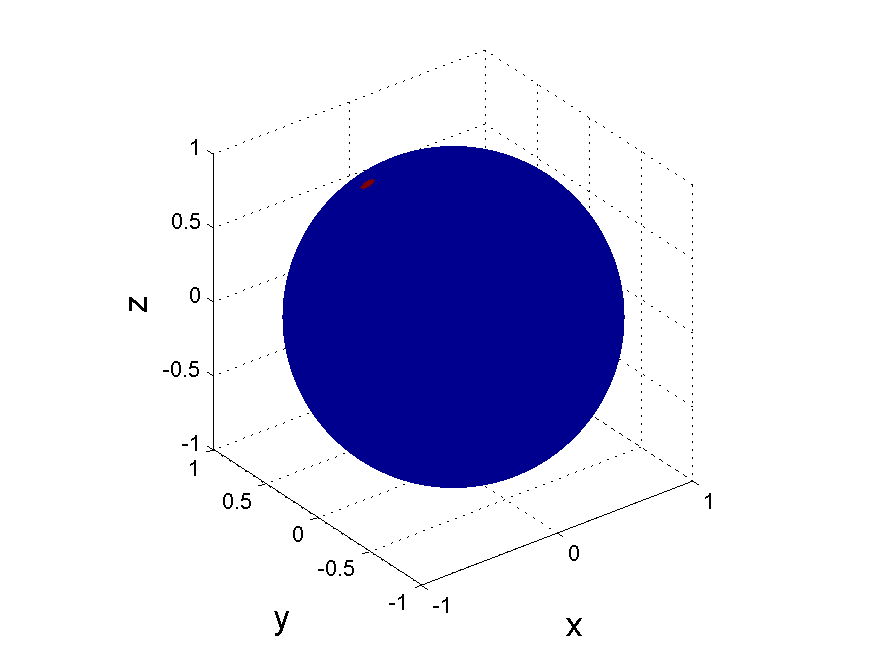
\includegraphics[width=0.45\textwidth]{kugel/Dkonstant/Kugel1_1.pdf}
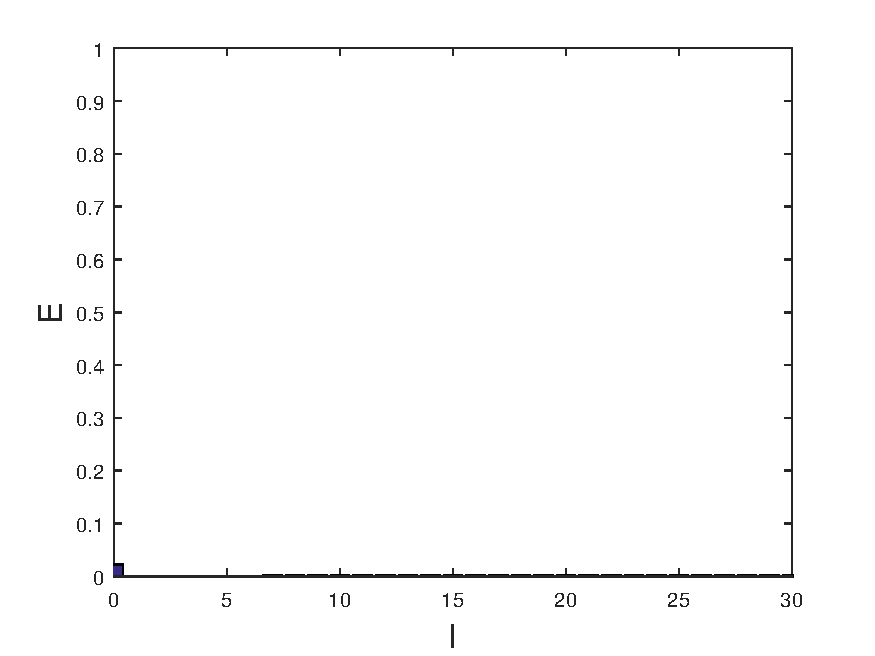
\includegraphics[width=0.45\textwidth]{kugel/Dkonstant/Kugel1_2.pdf}
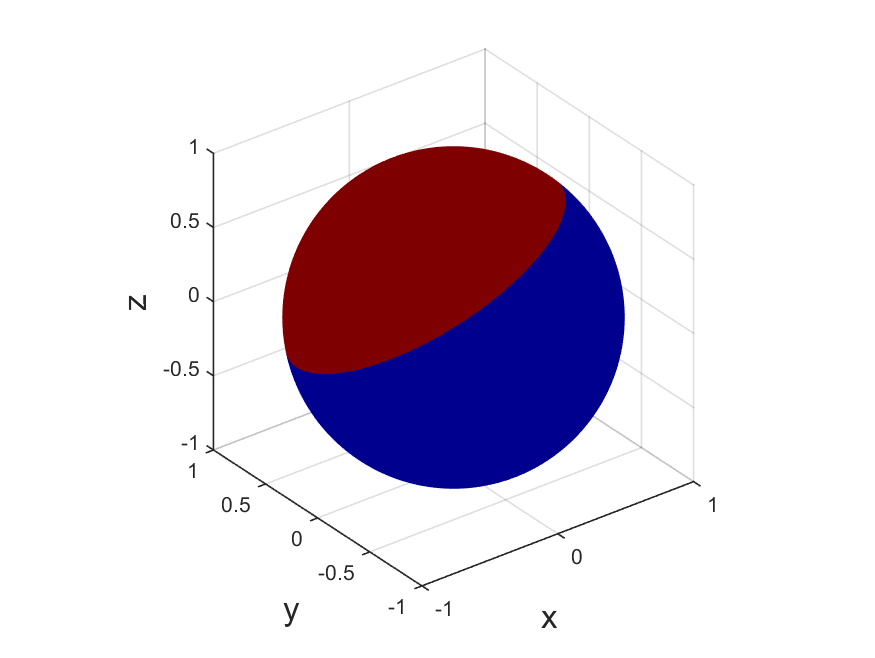
\includegraphics[width=0.45\textwidth]{kugel/Dkonstant/Kugel2_1.pdf}
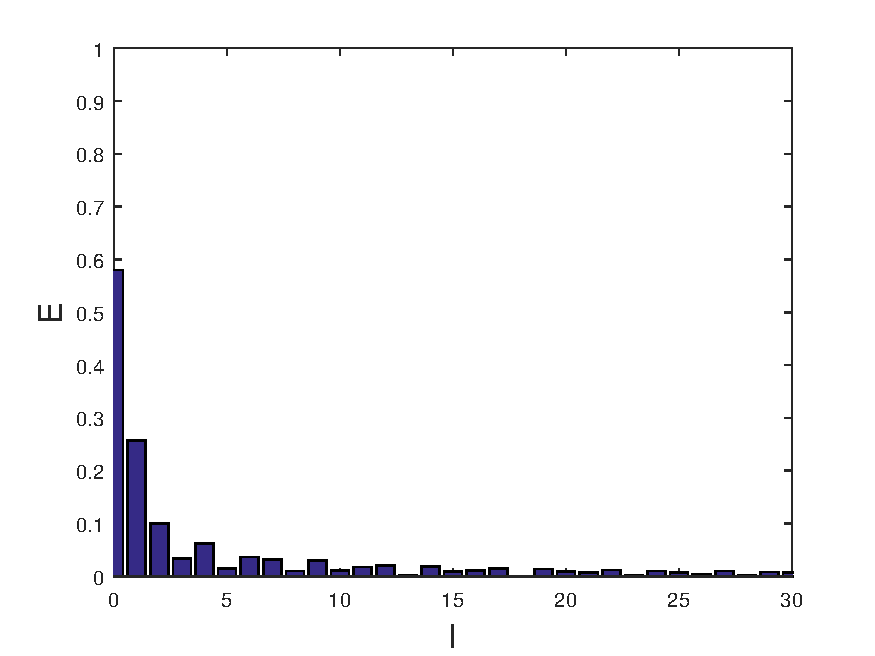
\includegraphics[width=0.45\textwidth]{kugel/Dkonstant/Kugel2_2.pdf}
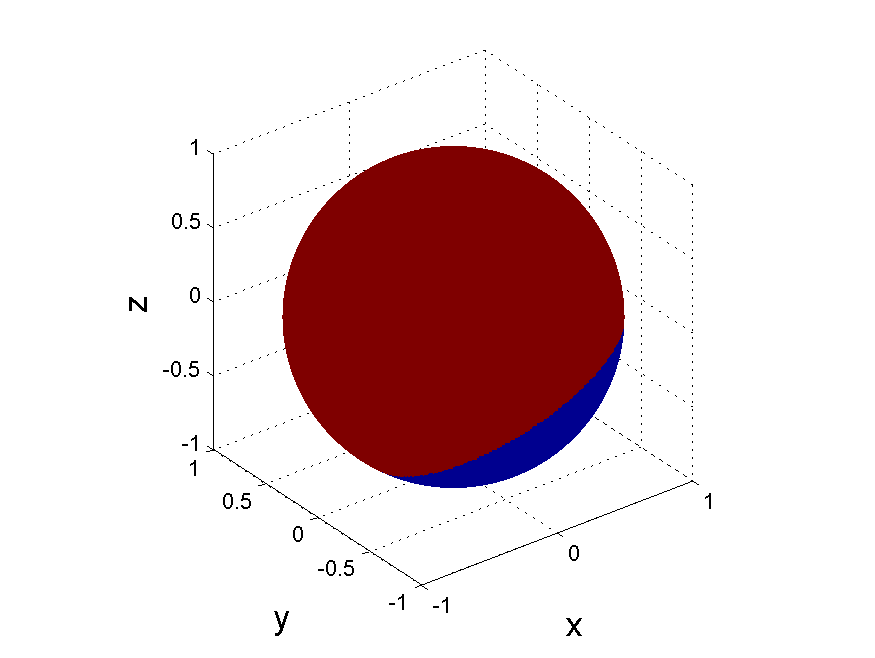
\includegraphics[width=0.45\textwidth]{kugel/Dkonstant/Kugel3_1.pdf}
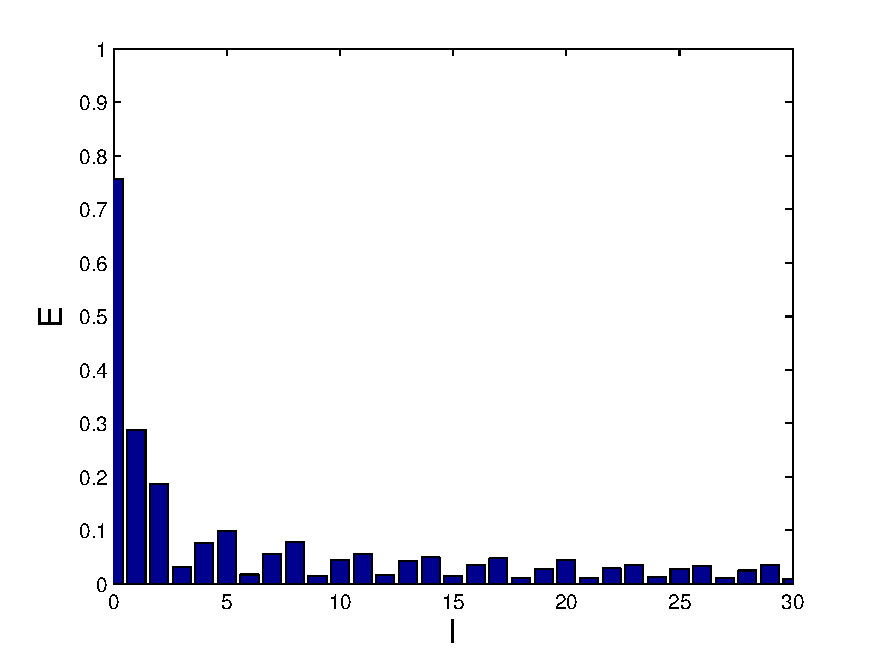
\includegraphics[width=0.45\textwidth]{kugel/Dkonstant/Kugel3_2.pdf}
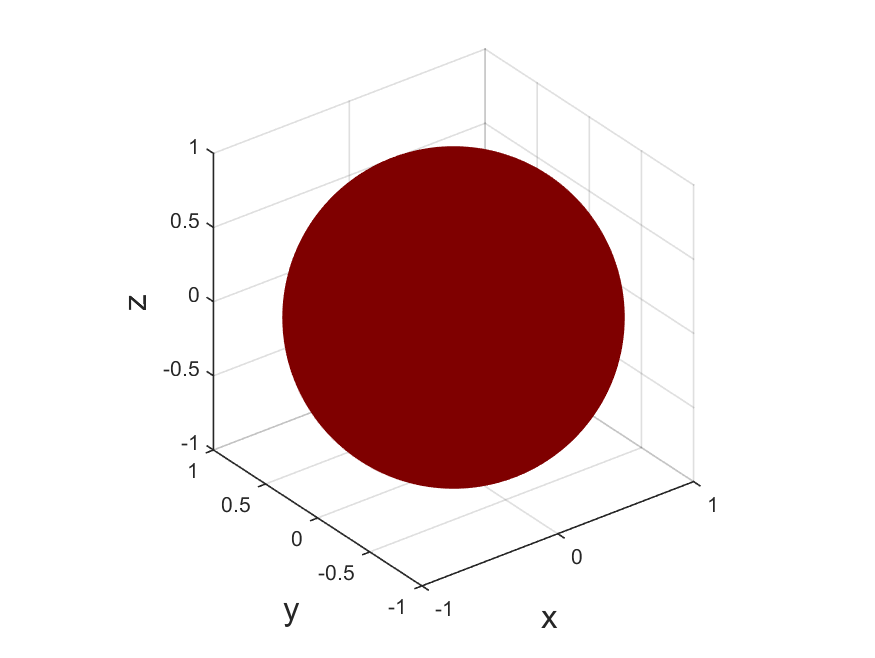
\includegraphics[width=0.45\textwidth]{kugel/Dkonstant/Kugel4_1.pdf}
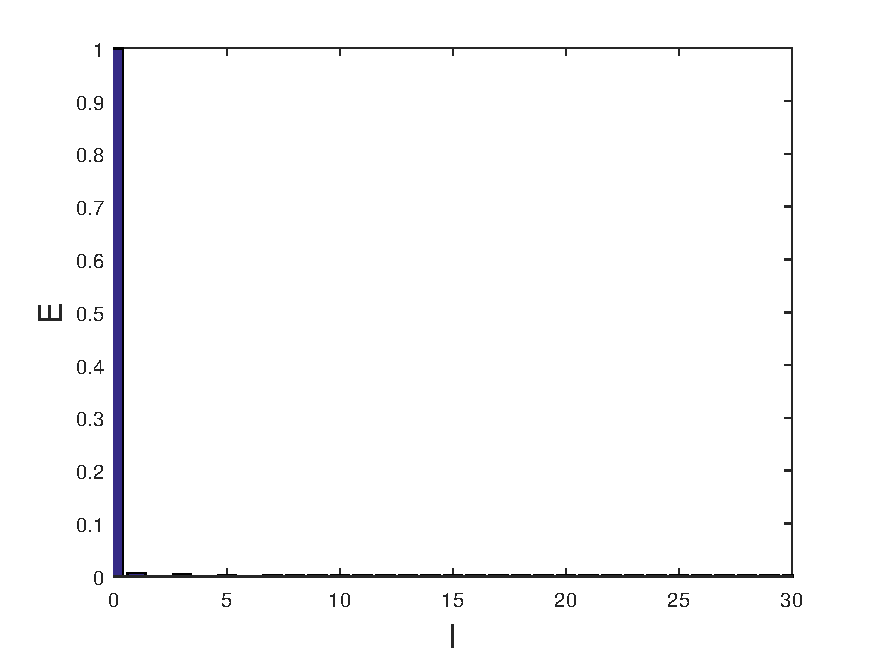
\includegraphics[width=0.45\textwidth]{kugel/Dkonstant/Kugel4_2.pdf}
%\caption{Titel??
\label{skript:Dirac1}%}
\end{figure}

\section{Gibbs-Ph"anomen}
\rhead{Gibbs-Ph"anomen}
Der gibbssche Effekt tritt immer dann auf, wenn eine Funktion 
Spr"unge aufweist. 
Bei der Original-Rechteckfunktion in Abbildung \ref{skript:Gibborg} 
kann man einen solchen Sprung sehen. Beim, mit den ersten 100
Fourier-Koeffizienten, rekonstruierten Rechtecksignal in 
Abbildung \ref{skript:Gibbsre} kann man erkennen, 
dass der Sprung nicht ganz so steil ist und es vor und nach dem 
Sprung "uberschwingt. 
Dieselben Effekte sind in Abbildung \ref{skript:Gibbs1} und 
Abbildung \ref{skript:Gibbs2} auch auf der Kugeloberfl"ache zu 
erkennen.
Mit n wird jeweils bezeichnet wie viele Koeffizienten f"ur die 
Rekonstruktion der Funktionen verwendet wurden.

\begin{figure}
\begin{minipage}[hbt]{0.5\textwidth}
\centering
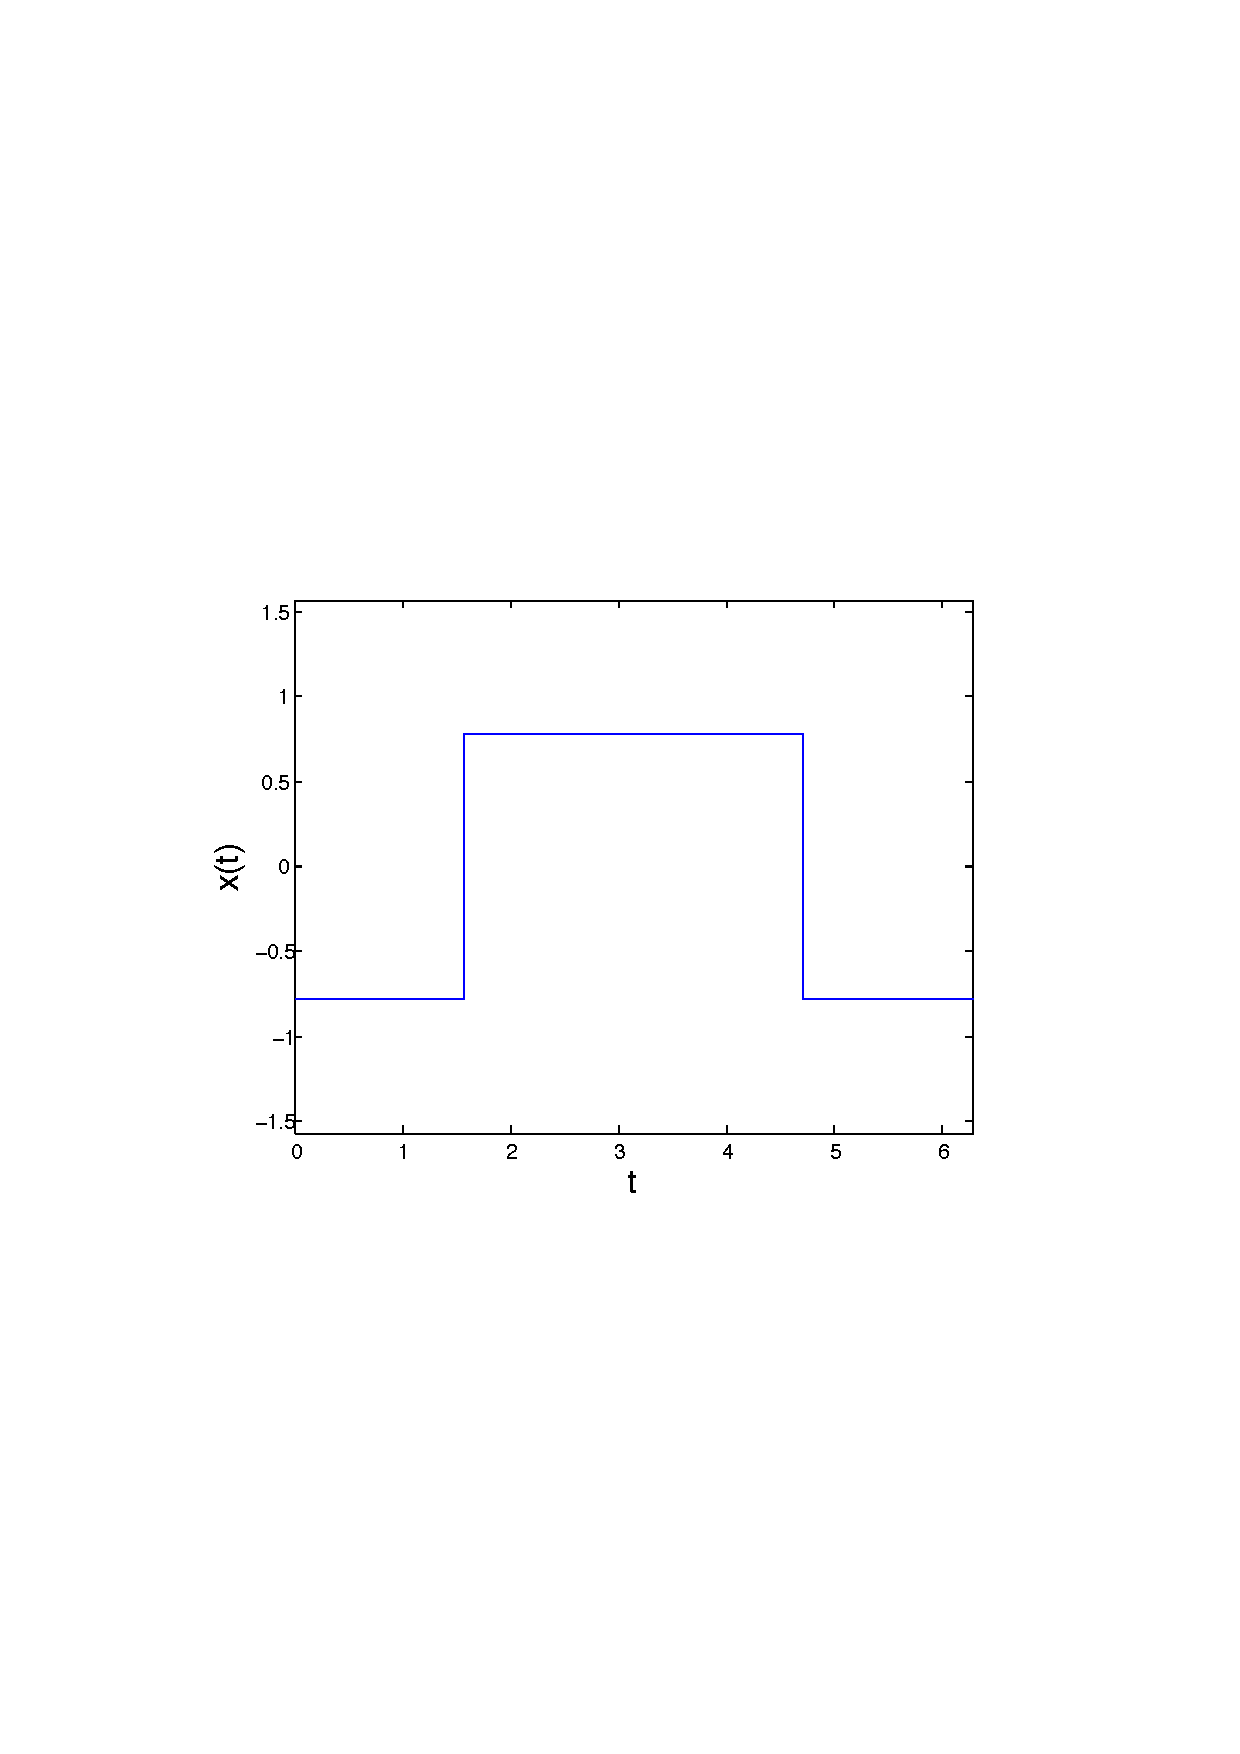
\includegraphics[width=1\textwidth]{kugel/Gibbs/Funktion.pdf}
\caption{Original-Rechteckfunktion}
\label{skript:Gibborg}
\end{minipage}
\hfill
\begin{minipage}[hbt]{0.5\textwidth}
\centering
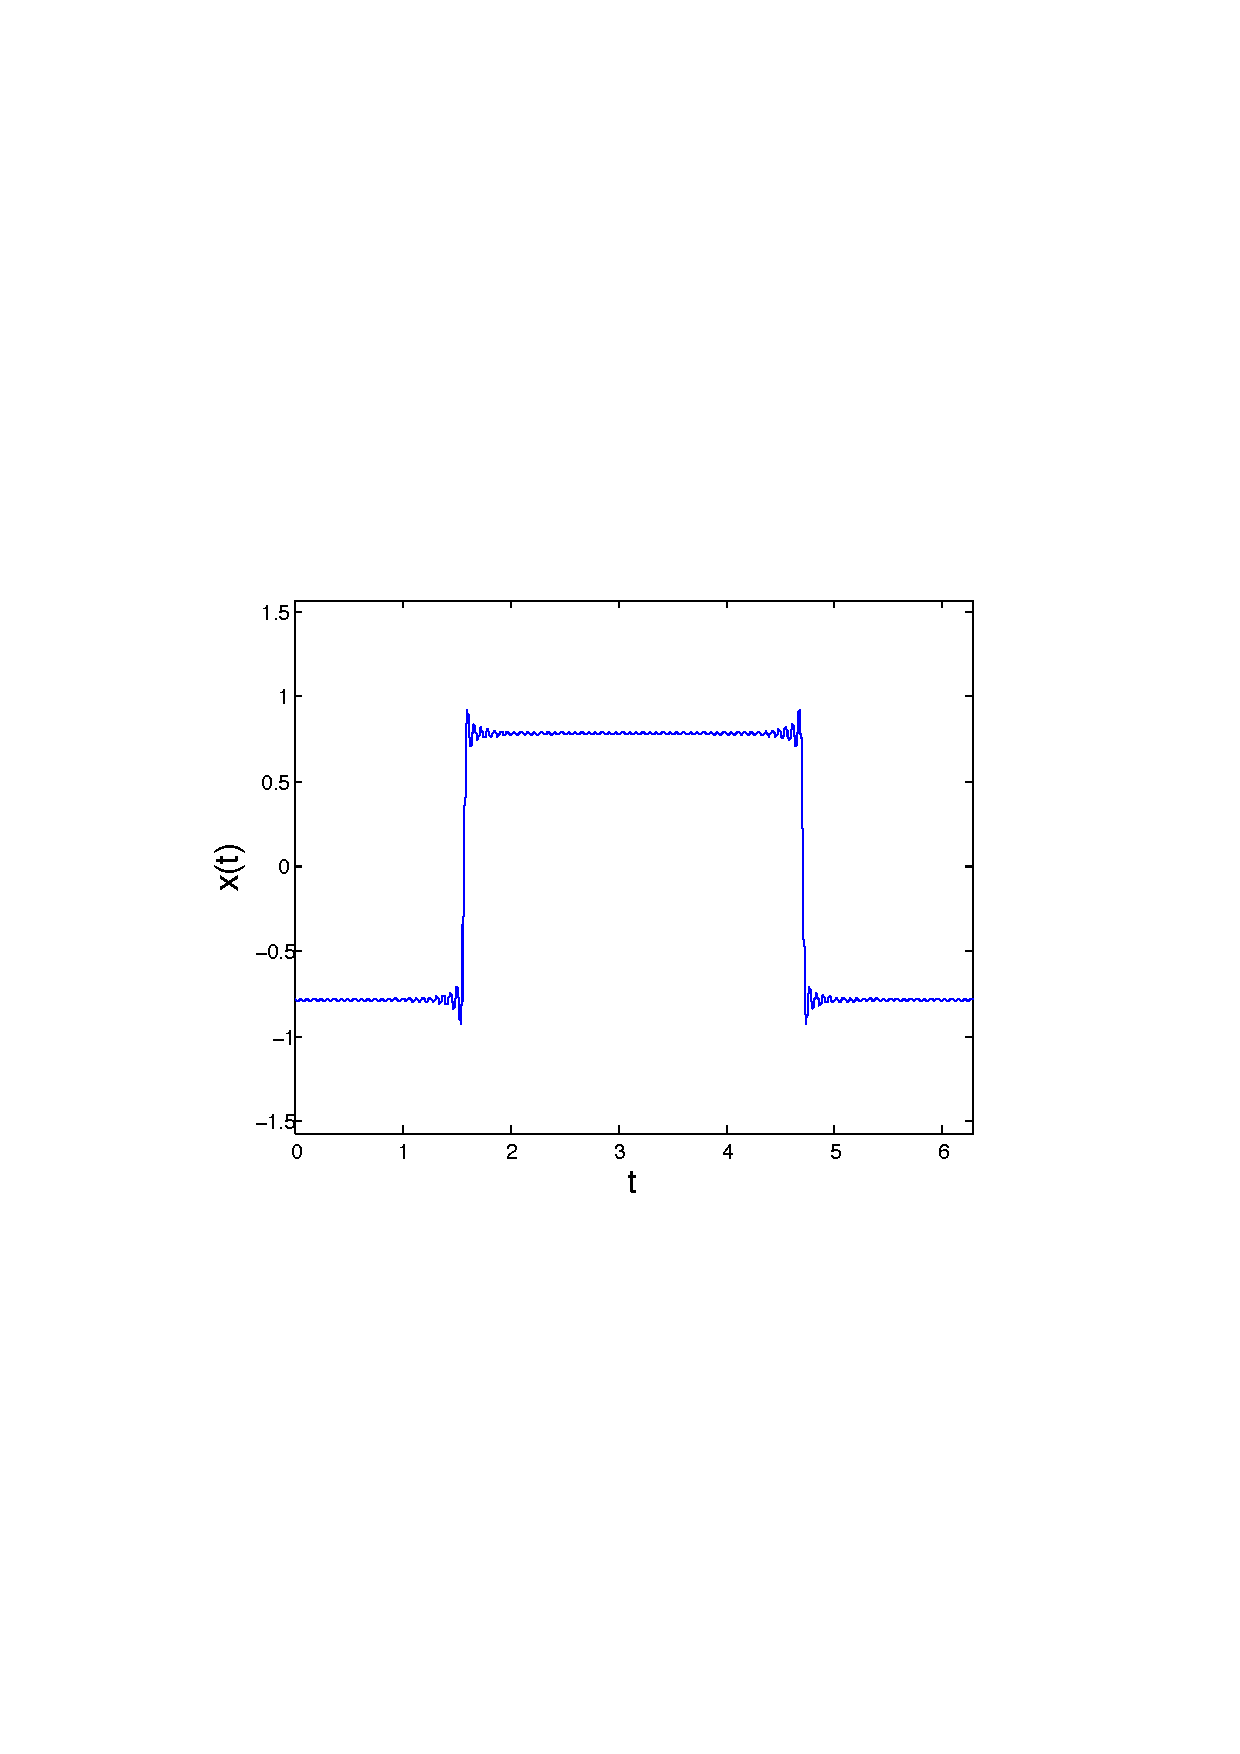
\includegraphics[width=1\textwidth]{kugel/Gibbs/Gibbs.pdf}
\caption{Rekonstruiertes Rechtecksignal}
\label{skript:Gibbsre}
\end{minipage}
\end{figure}

\begin{figure}% Gibbsscher-Effekt
\centering
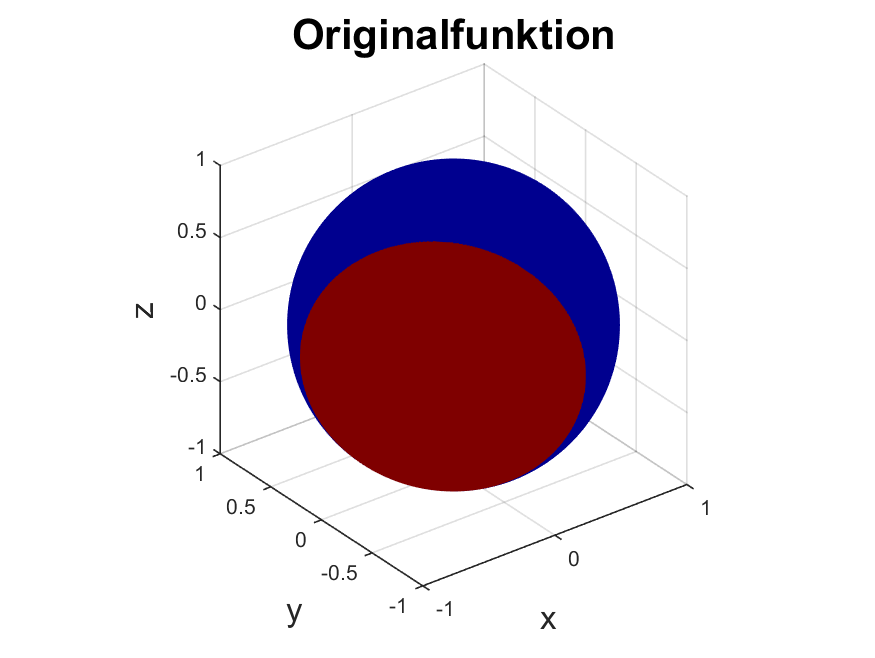
\includegraphics[width=0.4\textwidth]{kugel/Gibbs/GibbsOriginalFunktion.pdf}
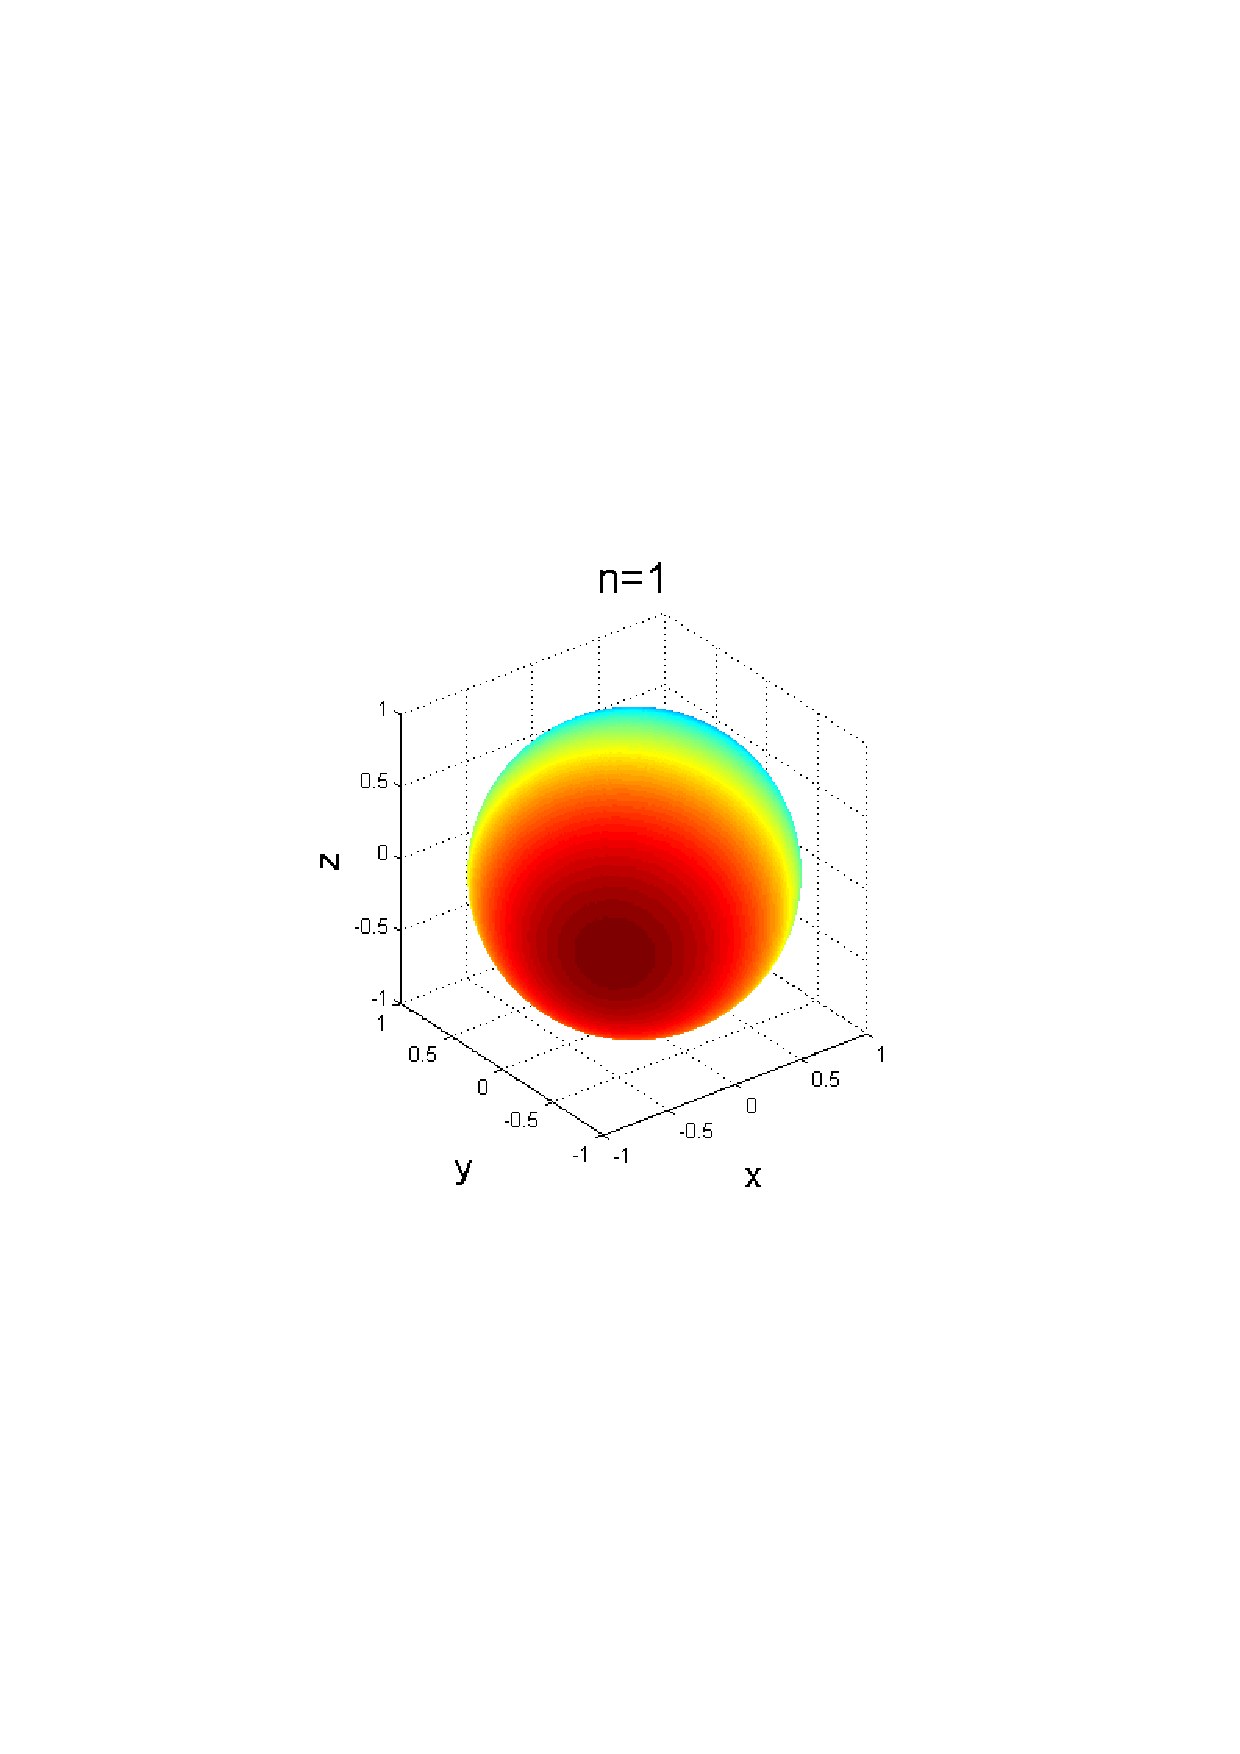
\includegraphics[width=0.4\textwidth]{kugel/Gibbs/GibbsN_1.pdf}
\includegraphics[width=0.4\textwidth]{kugel/Gibbs/GibbsN_2.pdf}
\includegraphics[width=0.4\textwidth]{kugel/Gibbs/GibbsN_3.pdf}
\includegraphics[width=0.4\textwidth]{kugel/Gibbs/GibbsN_4.pdf}
\includegraphics[width=0.4\textwidth]{kugel/Gibbs/GibbsN_5.pdf}
\caption{Gibbsscher-Effekt $n=1$ bis $n=5$
\label{skript:Gibbs1}}
\end{figure}

\begin{figure}% Gibbsscher-Effekt
\centering22
\includegraphics[width=0.4\textwidth]{kugel/Gibbs/GibbsOriginalFunktion.pdf}
\includegraphics[width=0.4\textwidth]{kugel/Gibbs/GibbsN_10.pdf}
\includegraphics[width=0.4\textwidth]{kugel/Gibbs/GibbsN_15.pdf}
\includegraphics[width=0.4\textwidth]{kugel/Gibbs/GibbsN_20.pdf}
\includegraphics[width=0.4\textwidth]{kugel/Gibbs/GibbsN_25.pdf}
\includegraphics[width=0.4\textwidth]{kugel/Gibbs/GibbsN_30.pdf}
\caption{Gibbsscher-Effekt $n=10$ bis $n=30$
\label{skript:Gibbs2}}
\end{figure}


\printbibliography[heading=subbibliography]
\end{refsection}